\part{Behavioral-Disease Model}
\label{part:the_model}
\chapter{Model development and justification}
\label{ch:why_new}
Because the main contribution of this thesis is the development of a new multi-system model, understanding the reasons that led to its development is crucial.
Otherwise, the reader might question: "Why not use an already developed and analyzed model?"

The primary answer lies in the observation made while studying the literature: the connection between empirical data and epidemiological models is often missing. Most works relating social and epidemiological aspects are purely theoretical models based on ad-hoc assumptions; probably, because constructing a framework grounded in empirical data related to individual behavior is challenging \cite{Nunner2021}, and, until the COVID-19 pandemic, data on this topic were scarce.

The availability of research such as the one conducted by Meta during the COVID-19 pandemic \cite{Astley_2021} serves as a major source of inspiration and data. This research allows exploration of different behaviors related to how people react to and manage the necessity of living with an infectious disease. It also provides this valuable information as a dynamic time series.

Often, what emerges from this data is the non-linear dynamic evolution of behavior. While many models do not incorporate this characteristic \cite{huys2010nonlinear}, this feature is here addressed.
\begin{figure}[ht]
	\centering
	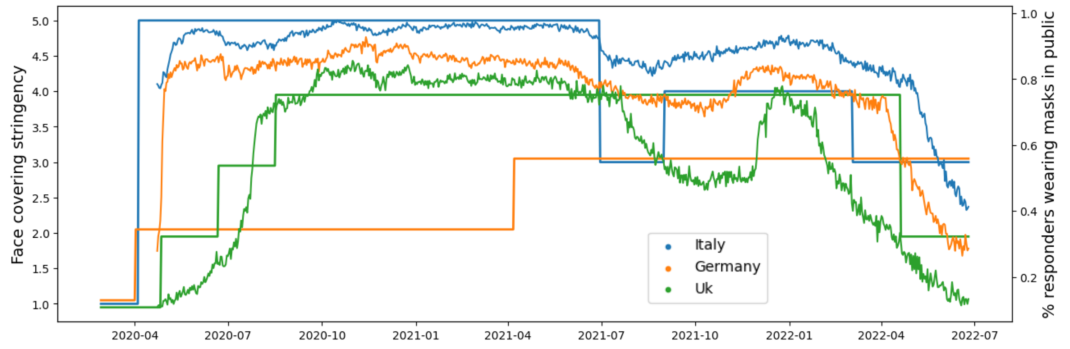
\includegraphics[width=0.8\linewidth]{1_corpo/figure/Fig2cut}
	\caption[Mask wearing evolution]{The evolution of mask wearing behaviors during the COVID-19 pandemic. Figure from \cite{Proverbio_Tex_2024}.}
	\label{fig:mask_wearing}
\end{figure}
The behavioral-epidemic mean-field model we developed aims to interconnect these two features, linking the theoretical framework with empirical evidence. Often, in other works, this connection is realized using proxy models that attempt to reconstruct agent behavior, spatial motion, or opinion datasets extrapolated, for instance, from social networks, as done in \cite{Anderson_2019,Zino_2021}. The problem with these approaches is that people's opinions do not always align with their actual behaviors, and the lack of a necessary and direct correlation between the two is another concept the model attempts to overcome.

For example, consider the evolution of mask-wearing behavior in different European countries during the COVID-19 pandemic, as shown in Figure \ref{fig:mask_wearing}. It is immediately evident that, at a certain point, there is a sharp increase in the use of this self-protective device, resembling a step function. This effect results from regulatory prescriptions introduced by authorities, and behaviors closely follow the evolution of these stringency measures.

Such phenomena have been incorporated into the model development using a coefficient parameter, $\psi$, to represent the effect of centralized interventions and modify the basic persuasion rate of different behaviors. Additional empirical evidence supporting the development of the model can be found in \cite{Proverbio_Tex_2024}. 

\begin{figure}[ht]
	\centering
	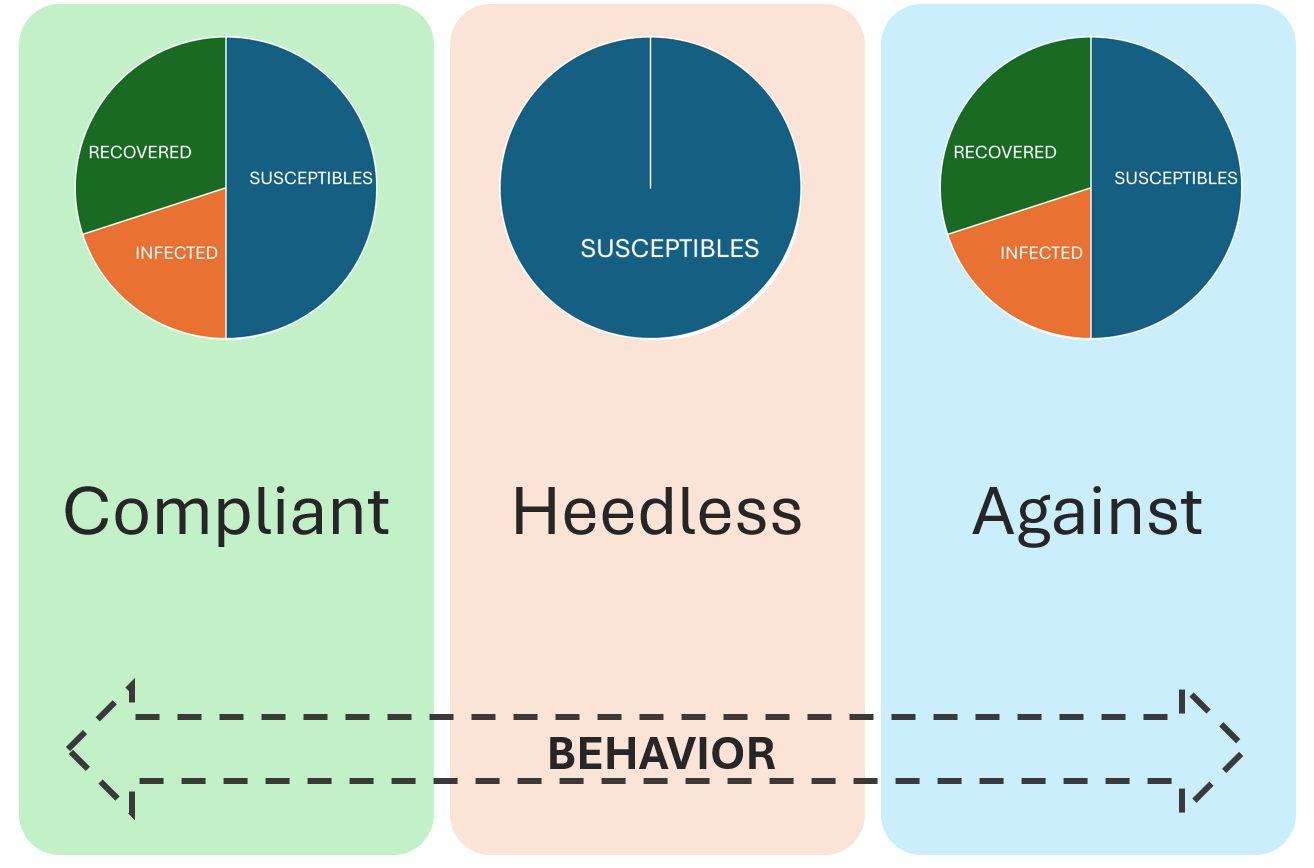
\includegraphics[width=0.6\linewidth]{1_corpo/figure/Model_behav_epidemic}
	\caption[Epi-behavior model]{Representation of the model with individuals divided into different behavioral categories, each of which can correspond to a specific disease state, except for the Heedless group, which is characterized solely by Susceptible individuals.}
	\label{fig:modelbehavepidemic}
\end{figure}

To introduce the model and begin its description, the next chapter first presents and analyzes the two layers that together form the complete model: a SIRS epidemic model and a behavioral model consisting of three compartments: Compliant, Against, and Heedless. Then, the full model is presented, described and analysed in Chapter \ref{ch:epi_behav_model}.
Then the full model is presented, described and analysed. 
The full model comprises seven compartments, as the heedless behavior is not possible for individuals that are infected or recovered. This assumption stems from the reasoning that it is highly improbable for an individual to act heedlessly when infected (unless, potentially, when completely asymptomatic). Figure \ref{fig:modelbehavepidemic} provides a compact representation of the population subdivision.

Infection can be transmitted across all three behavioral groups, but the Compliant group is more cautious. A parameter, $\rho$, models their reduced probability of being infected, while another parameter, $\epsilon$, accounts for their compliance with self-isolation while infectious. This reduces the number of infected Compliant individuals ($I_C$ in the model equations that will be presented in the next chapter \ref{ch:epi_behav_model}) contributing to new infections in the epidemic layer.

Behavior is "transmitted" through peer-to-peer influence with strenght parameters ($k_i, i = \,1,...,6$), with $i$ the number of compartments either Compliant or Against, and fatigue parameters ($\lambda_i$) are included to model the dropout rate caused by the difficulty of maintaining a certain behavior over time.

For the epidemic components of the model, classical coefficients are used: $\beta$ (transmission rate), $\gamma$ (recovery rate), and $\delta$ (immunity waning rate).
 

\chapter{Epidemic model and Behavioral model alone}
\label{ch:model_alone}

To develop a multi-system model that combines an epidemiological layer with a behavioral one, we first present the dynamics of each layer independently. We briefly introduce the SIRS model, focusing primarily on the reasons for its selection. Then, the Heedless, Compliant, Against behavioral model is introduced, simulated, and analyzed. Understanding the underlying dynamics of this model is crucial for gaining insight into the complex interactions that emerge within the multi-system model.


\section{SIRS model}
\label{sec:SIRS}
To describe the epidemic evolution, a  SIRS model is implemented. It is an extension of the most famous SIR discussed in Section \ref{subsec:SIR}. Its main addition is the possibility for individuals to become again susceptible after a certain period of time beyond the end of the infection due to waning immunity. There are four main characteristic parameters in this model:
\begin{itemize}
	\item $\beta$ is the transmission rate parameter for person-to-person
	contact.
	\item $\gamma$ is the recovery rate.
	\item  $\delta$ is the rate at which immunity wanes following recovery.
	\item  $\mathcal{R}_0$ is the reproduction number, similar conceptually to the one presented in SIR model, but function of $\beta, \gamma$, and also $\delta$. 
\end{itemize}
A SIR-like model is chosen because of its ability to describe diseases like COVID-19; the literature provides numerous examples that use this model \cite{Dehning_2020, Li2022}. The SEIR model could also be a viable choice due to the relevance of the "Exposed" compartment, which effectively captures the disease progression for infections such as COVID-19. In these cases, an incubation period occurs after exposure before symptoms appear and the individual becomes contagious. However, this compartment was excluded because it has been shown \cite{Dehning_2020} that a simpler SIR model can still accurately represent the disease dynamics. When comparing model simulations with real data, a delay can be incorporated to account for the lag between symptom onset, testing, and reporting. This delay reflects the time needed for symptoms to manifest, conduct testing, and report cases to relevant authorities.
The differential system of equations describing the model are
\begin{equation}
	\label{eq:SIRS_eq}
	\begin{cases}
		\frac{ds}{dt} = -\beta s i + \delta r \\
		\frac{di}{dt} = \beta s i -  \gamma i \\
		\frac{dr}{dt}= \gamma i -  \delta r\\
	\end{cases}
\end{equation}
with $s(0) = s_0 \ge 0$, $i(0) \ge 0$ and $r(0) = 0$. The mass conservation assumption holds so $s(t)+i(t)+r(t) =1$.
The model includes the possibility of reinfection, which is important when studying long-term scenarios. Considering the effect of individual behavior on disease progression, two critical phases are hypothesized to influence this evolution: the initial stages of the epidemic and the period following the first peak.

In the initial stages, the SIRS model behaves similarly to a typical SIR model, because reinfection is unlikely to occur in a short time frame. However, over time, as reinfections become possible, individual attitudes and behaviors increasingly impact the disease spread.

\begin{figure}[ht]
	\centering
	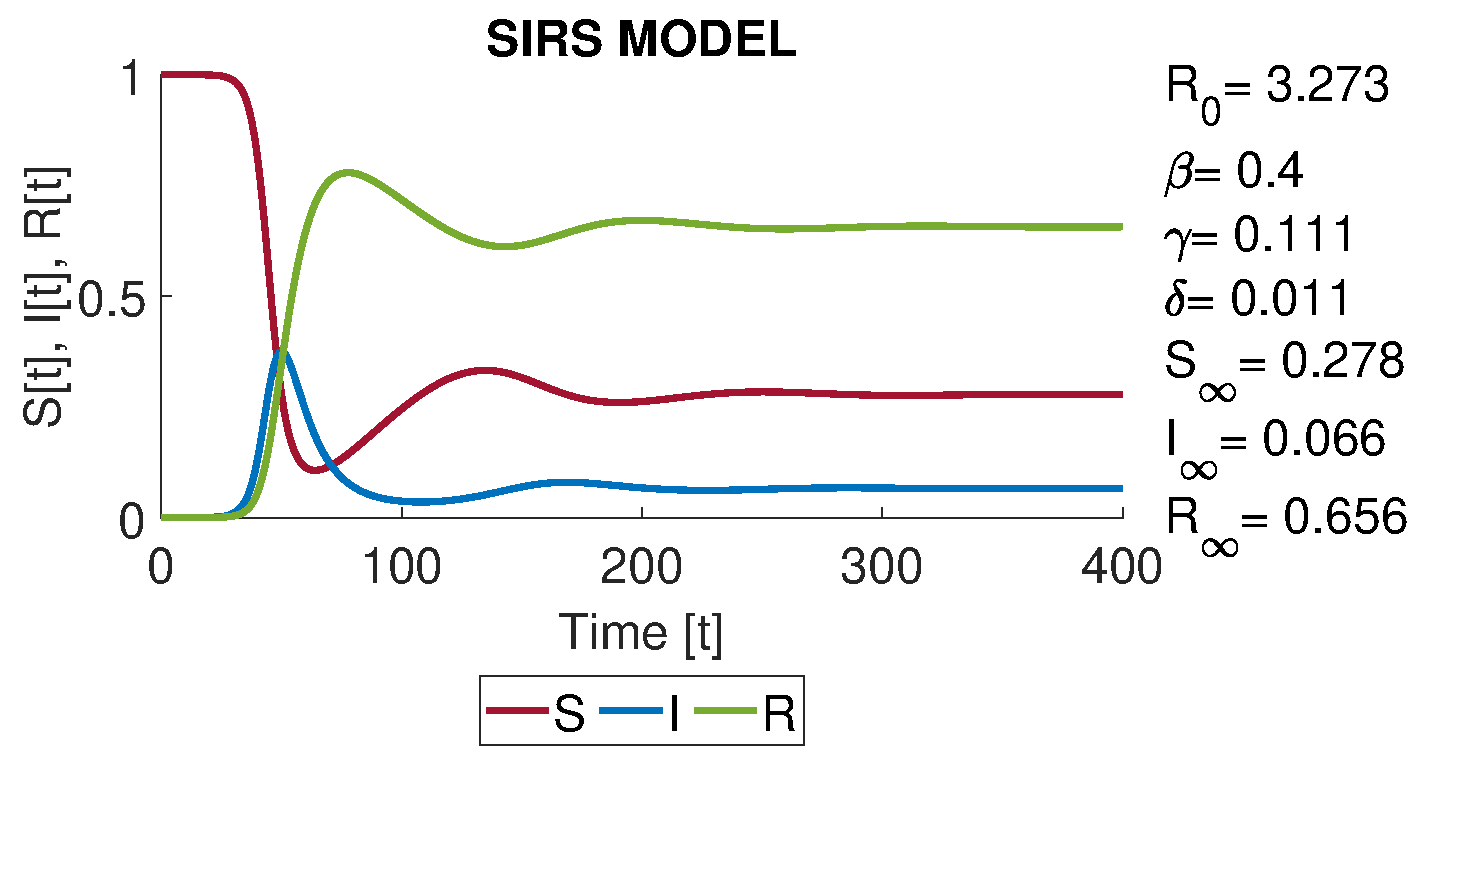
\includegraphics[width=0.6\linewidth]{1_corpo/figure/r0/sirs_figure}
	\caption[SIRS simulation]{Simulation of the SIRS model. The parameters of the model, which meaning is presented in section \ref{sec:sir_presentation}, are chosen to resemble those of the initial stages of the COVID-19 pandemic \cite{data_R0_covid} and are the same as those used for simulations with the full epi-behavioral model.}
	\label{fig:sirsfigure}
\end{figure}

\section{Behavioural model}
\label{sec:behavioral_model}

The development of the behavioral model builds on several works already presented in the literature. In particular, the following mechanisms are considered to be the most relevant:
\begin{itemize}
	\item The competition between two opposing behaviors/opinions, driven by peer pressure \cite{Epstein_2021}. The implementation is inspired by the Unaware-Aware-Unaware opinion model class \cite{Zuo2022, Peng2021}, refer to Section \ref{subsec:individual_state} and \ref{subsec:multisystem_models}, for how the compartments are linked together and for the idea of social pressure between individuals.
	
	\item Non-compliance viewed as a form of social contagion \cite{Bongarti2023}.
	 
	\item The fatigue mechanism, due to which maintaining a certain behavior for long leads to a spontaneous loss of compliance \cite{Epstein_2021}.
\end{itemize}

To integrate all these aspects into a mean-field model, the first step is to define the compartments used to segment the population. The population is divided into three compartments: Heedless, Compliant, and Against, denoted respectively as H, C, and A. The meaning of each compartment is as follows:
\begin{itemize}
	\item[\textbf{$H$:}] Individuals who behave without much regard for guidelines and are careless about the risks associated with the infection.
	\item[\textbf{$C$:}] Individuals who actively seek to avoid becoming infected or spreading the virus by following guidelines and taking precautions.
	\item[\textbf{$A$:}]Individuals who do not consider the infection a risk to their safety and do not use protection or modify their behavior during the epidemic. They disregard risk-mitigating guidelines and do not align with safer behaviors as the epidemic unfolds.
\end{itemize}

\subsubsection{Initial conditions}
As an initial condition, the hypothesis is that most of the population is in the Heedless compartment. This assumption is based on the idea that when a new disease emerges, it is poorly understood, and the population has limited information about it. The hypothesis is that people in the Heedless compartment may be clueless about the risks of becoming infected. This lack of knowledge causes them to maintain their usual behavior, making them susceptible to infection. This assumption is also supported by data and literature \cite{Usher_2020}. As an example of this initial configuration, the case of COVID-19 in Italy is considered. In the early stages of its spread, when the disease was primarily affecting China, it was not viewed as a significant threat by most of the population in Western countries. It was perceived as a distant issue affecting a faraway nation. Therefore, when the epidemic reached Europe and Italy, both the population and the government were caught off guard. There was an initial delay in the implementation of countermeasures, as well as in the dissemination of reliable information about the disease progression to the general public.

In addition, there are two opposing behavioral groups, which in the initial phase of the dynamic comprise a small fraction of the population: Compliant and Against.

The Compliant group actively seeks to reduce their chances of becoming infected or infecting others. They adopt self-protection measures such as wearing face masks, sanitizing their hands, and voluntarily limiting their presence in public spaces to reduce contact with others.

In contrast, the Against group consists of individuals who, for personal reasons—such as anti-scientific beliefs, low trust in policymakers, or other concerns—do not take action to minimize their chances of infection or the possibility of infecting others. This category encompasses phenomena such as: 
\begin{itemize} 
	\item vaccine denial; 
	\item misinformation spread; 
	\item denial of the existence of the disease; 
	\item distrust of doctors and government policies. 
\end{itemize}

The inclusion of the Against compartment stems from the fact that, especially in the early stages of a new disease outbreak, there is often a lack of reliable knowledge. As documented by \cite{McCormack_2020}, this can lead to the spread of false beliefs in the population. It has also been demonstrated \cite{owid-vaccine-skepticism} that misinformation, especially when associated with fear, can have lasting effects. A notable example is the belief that the measles, mumps, and rubella (MMR) vaccine can cause developmental disorders in children. Despite the fact that the original publication making this claim has been scientifically discredited \cite{wakefield1998retracted}, this idea remains popular and has contributed to a rise in vaccine skepticism \cite{owid-vaccine-skepticism}.

\subsubsection{Social contagion dynamic}
The evolution of the model is governed by two principal mechanisms: \begin{itemize} 
	\item Heedless individuals transition to either Compliant or Against compartments. 
	\item Compliant and Against individuals return to the Heedless compartment. 
\end{itemize}
\begin{figure}[ht]
	\centering
	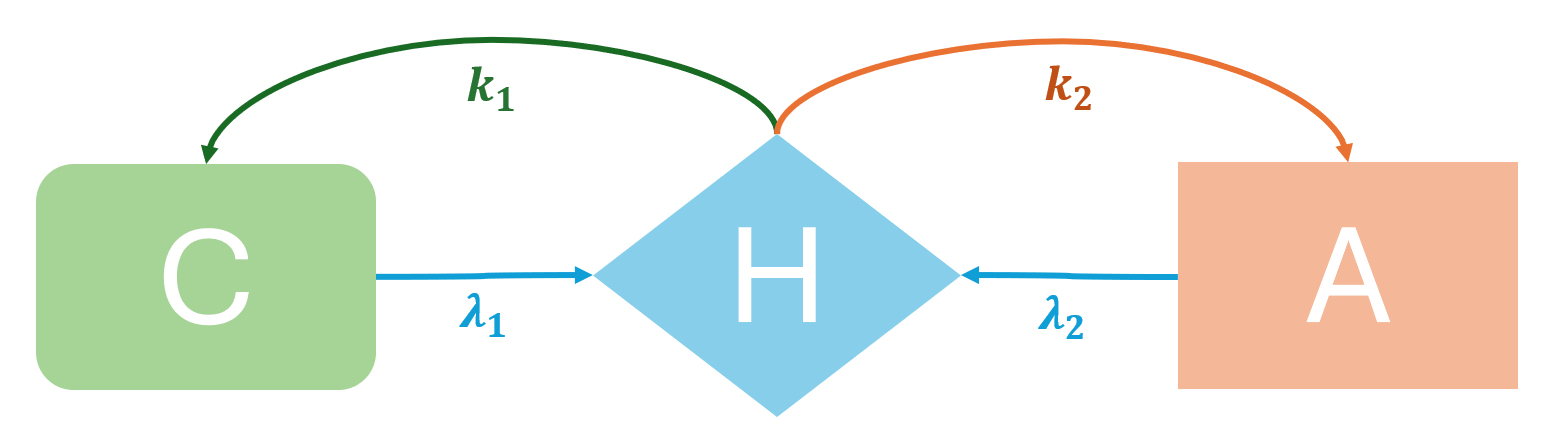
\includegraphics[width=0.72\linewidth]{1_corpo/figure/behavior_model_figure}
	\caption[Behavior model]{The figure visualizes the developed behavioral model, featuring three compartments: Heedless, Compliant, and Against, abbreviated as H, C, and A. The arrows indicate the inflows and outflows between these compartments.}
	\label{fig:behaviormodelfigure}
\end{figure}
The first mechanism is driven by peer pressure: the size of each group and its level of persuasiveness are the parameters that govern this process. It is mathematically modeled similarly to person-to-person disease transmission, as seen in the SIR-like mean-field model described in Section \ref{subsubsec:p2p_transmission}. Instead, the return to the Heedless compartment is modeled as a spontaneous decay process: individuals naturally leave the Compliant and Against compartments and return to Heedless, transitioning spontaneously depending on the level of fatigue associated with maintaining the behavior.The flow between an intermediate compartment, represented by $H$, rather than a direct transition between $A$ and $C$ (and vice versa), is a modeling choice stemming from the idea that heedlessly can, when a new disease appears, signify lack of awareness about it. Over time, it can represent instead the state of people after a period of coexistence with the disease, where the fatigue of maintaining compliance increases, or when indifference toward the disease grows.
To describe these transitions, different coefficients are introduced. The $k_1$ and $k_2$ are persuasion rates, while $\lambda_1$ and $\lambda_2$ represent fatigue rates. Their meanings are as follows: \begin{itemize} 
	\item $k_1$: persuasion rate from Heedless to Compliant; 
	\item $k_2$: persuasion rate from Heedless to Against; 
	\item $\lambda_1$: rate at which the Compliant behavior is abandoned due to fatigue; 
	\item $\lambda_2$: rate at which the Against behavior is abandoned due to fatigue. 
\end{itemize}

The resulting differential equations describing the model dynamic are:
\begin{equation}
	\label{eq:behavioural_eq}
	\begin{cases}
		\dot{H} = -k_1 H C - k_2 H A + \lambda_1 C + \lambda_2 A \\
		\dot{C} = k_1 H C -  \lambda_1 C \\
		\dot{A} = k_2 H A -  \lambda_2 A\\
	\end{cases}
\end{equation}
We assume population mass conservation, meaning that the relationship $H + C + A = 1$ holds. Additionally, the initial conditions described in the previous section are translated as follows:
\begin{equation}
	\begin{cases}
		H(0) = 1 - C_0 - A_0\\
		C(0) = C_0 > 0\\
		A(0) = A_0 > 0\\
	\end{cases}
\end{equation}

\subsubsection{Behavior conversion number}

To simplify the understanding of the system underlying dynamics, an analogy can be drawn with the reproduction number in epidemic models. By examining the system equations \eqref{eq:behavioural_eq}, a relationship can be identified. From both the second and third equations, we can isolate the two coefficients (specifically $k_1 , \lambda_1 $, and  $k_2 , \lambda_2 $)  and derive a new parameter, called "Behavior Conversion Rate", $\mathcal{B}$. This rate is the result of the ratio between the persuasion rate and the fatigue decay rate, and can be viewed as a measure of the transmission potential of social contagion. The general formula to calculate it is:
\begin{equation}
	\mathcal{B}_i =\frac{ k_i }{\lambda_i}  \qquad \text{with } i = 1, \text{or } 2.
	\label{eq:behave_rate}
\end{equation}
In the model presented here, $\mathcal{B}_1$ represents the Behavior Conversion Rate associated with the Compliant compartment, while $\mathcal{B}_2$, is associated with the Against compartment. The results of different numerical simulations are now displayed to demonstrate how the relationship between these two values influences the evolution of social contagion.

\subsection{Model simulation}
To represent different dynamics, four main cases are now presented. The coefficient values have been set appropriately to highlight different interesting situations in which the system can evolve.

\begin{itemize}
	\item[I] case: $\mathcal{B}_1, \mathcal{B}_2 <1$, $\mathcal{B}_1 >  \mathcal{B}_2$, and $\lambda_1 > \lambda_2$.
	\item[II] case: $\mathcal{B}_1, \mathcal{B}_2 >1$, $\mathcal{B}_1 =  \mathcal{B}_2$, and $\lambda_1 < \lambda_2$.
	\item[III] case: $\mathcal{B}_1, \mathcal{B}_2 >1$, $\mathcal{B}_1 >  \mathcal{B}_2$, and $\lambda_1 = \lambda_2$.
	\item[IV] case: $\mathcal{B}_1, \mathcal{B}_2 >1$ and $\mathcal{B}_1 >  \mathcal{B}_2$, and $\lambda_1 < \lambda_2$.
\end{itemize}

The values $k_1$ and $k_2$ can be calculated from the formula of $\mathcal{B}_1$ and $\mathcal{B}_2$.

Figure \ref{fig:model__behavior_sim_1}a shows that, when both Behavior conversion numbers are less than one, social contagion does not spread: even though, in this case, the Compliant and Against compartments together represent $60\%$ of the total population at the beginning of the simulation, they clearly tend to zero over time. In contrast, Figure \ref{fig:model__behavior_sim_1}b shows the case where the two $\mathcal{B}$ values are equal and greater than one. To emphasize the importance of the relations between fatigue and persuasion rate, it is shown that, even if the conversion numbers are equal, (i.e. $k_2$  is lower than $k_1$=), the Compliant compartment becomes the majority group by the end of the simulation. Here the Against do not tend to zero, but there is a rather stable flow between the Compliant and Against compartments, through the Heedles state, such that
none of the compartments becomes empty.

\begin{figure}[ht]
	\centering
	\subfloat[][\emph{$\mathcal{B}_1, \mathcal{B}_2 <1$, $\mathcal{B}_1 >  \mathcal{B}_2$, and $\lambda_1 > \lambda_2$.}]
	{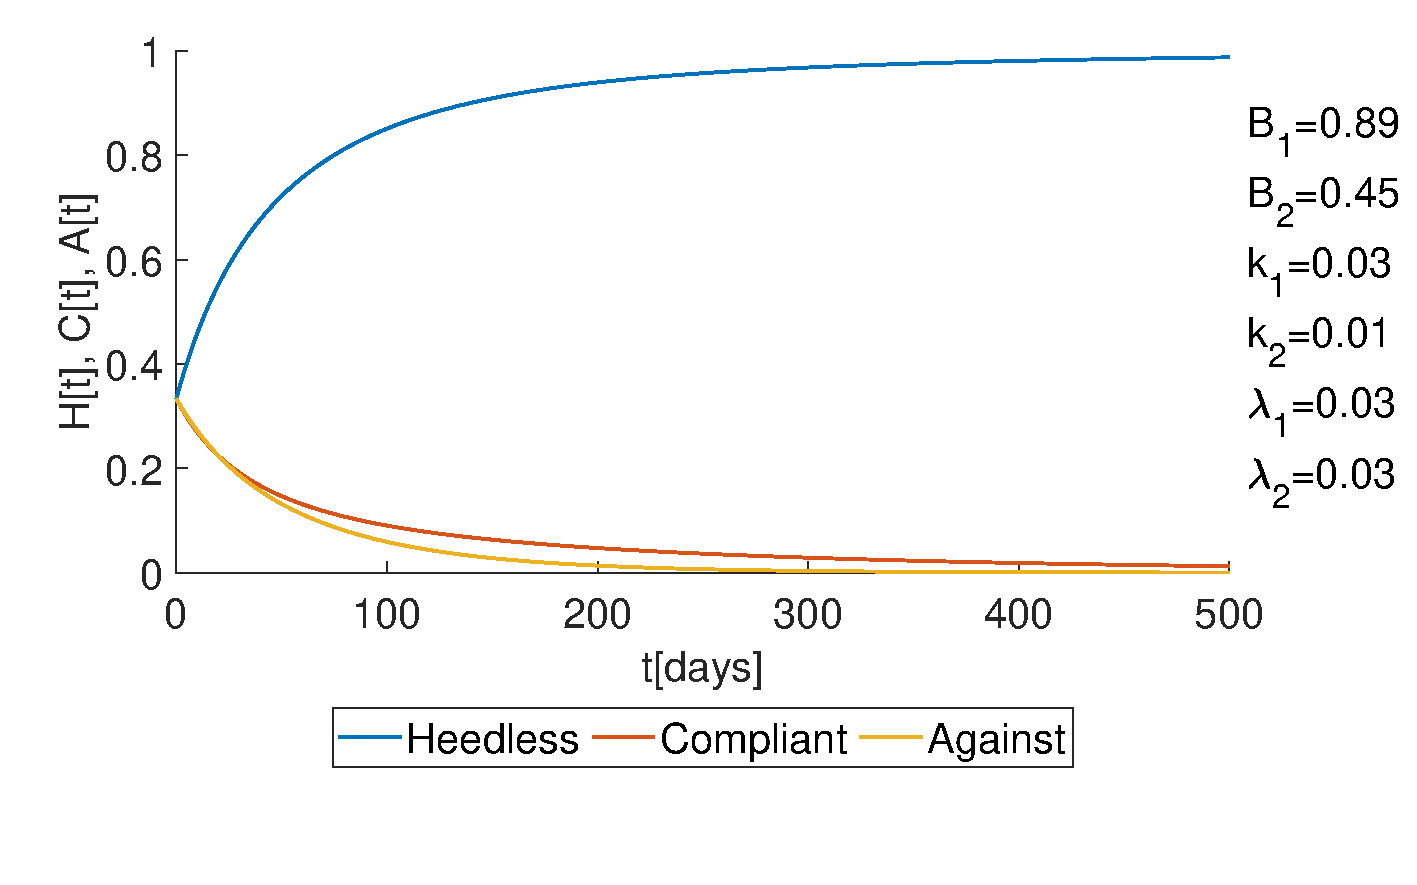
\includegraphics[width=0.48\linewidth]{1_corpo/figure/behavioural_equilibrium/behavior_B1_B2_less_1}} \quad
	\subfloat[][\emph{$\mathcal{B}_1, \mathcal{B}_2 >1$, $\mathcal{B}_1 =  \mathcal{B}_2$, and $\lambda_1 < \lambda_2$.}]
	{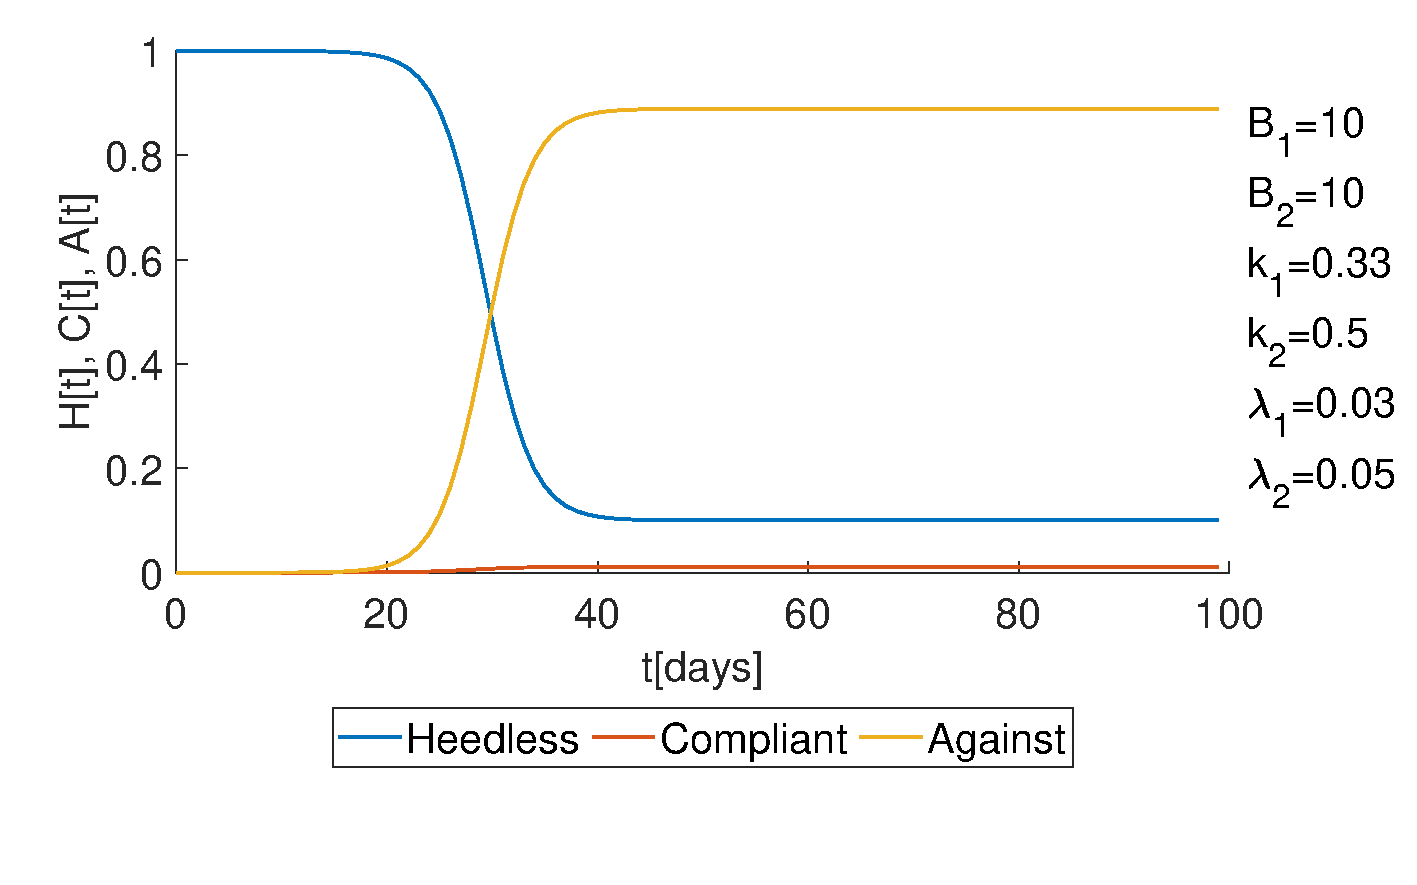
\includegraphics[width=0.48\linewidth]{1_corpo/figure/behavioural_equilibrium/behavior_B1_equal_B2}} \\
	\caption[Behavioural model simulation first]{Behavioral system dynamics first two cases (I and II). In the left panel there is the case in which both $\mathcal{B}_1$,$\mathcal{B}_2$ are less than one. The system tends to an equilibrium in which all individuals tends to the $H$ state. In the right panel, instead the case in which the conversion number are equal, but because $k_1 > k_2$ the Compliant variable becomes greater than the Against one.}
	\label{fig:model__behavior_sim_1}
\end{figure}
\label{subsec:model_behav}

Figure \ref{fig:model__behavior_sim_2} illustrates two other interesting scenarios. On the left, we observe the dynamics when one of the $\mathcal{B}$ values is greater than the other, and both $\lambda$ values are the same: the variable with the largest $\mathcal{B}$ becomes dominant. It is straightforward to understand that this dynamic would also occur if, with the same values of $\mathcal{B}$, the $\lambda$ of the dominant behavior were greater than the other, as a larger $\lambda$ would be compensated by  a higher $k$ (persuasion rate). The right panel, however, presents a particularly intriguing situation. Here, $\lambda_1$ < $\lambda_2$, combined with $k_2 > k_1$, leads to an initial rapid spread of the Against group, even though $\mathcal{B}_2 < \mathcal{B}_1$! It is only after some time that the system evolves to the final equilibrium, which is the same as in the left scenario, as the $\mathcal{B}$ values are the same in both simulations.

\begin{figure}[h]
	\centering
	\subfloat[][\emph{$\mathcal{B}_1, \mathcal{B}_2 >1$, $\mathcal{B}_1 >  \mathcal{B}_2$, and $\lambda_1 = \lambda_2$.}]
	{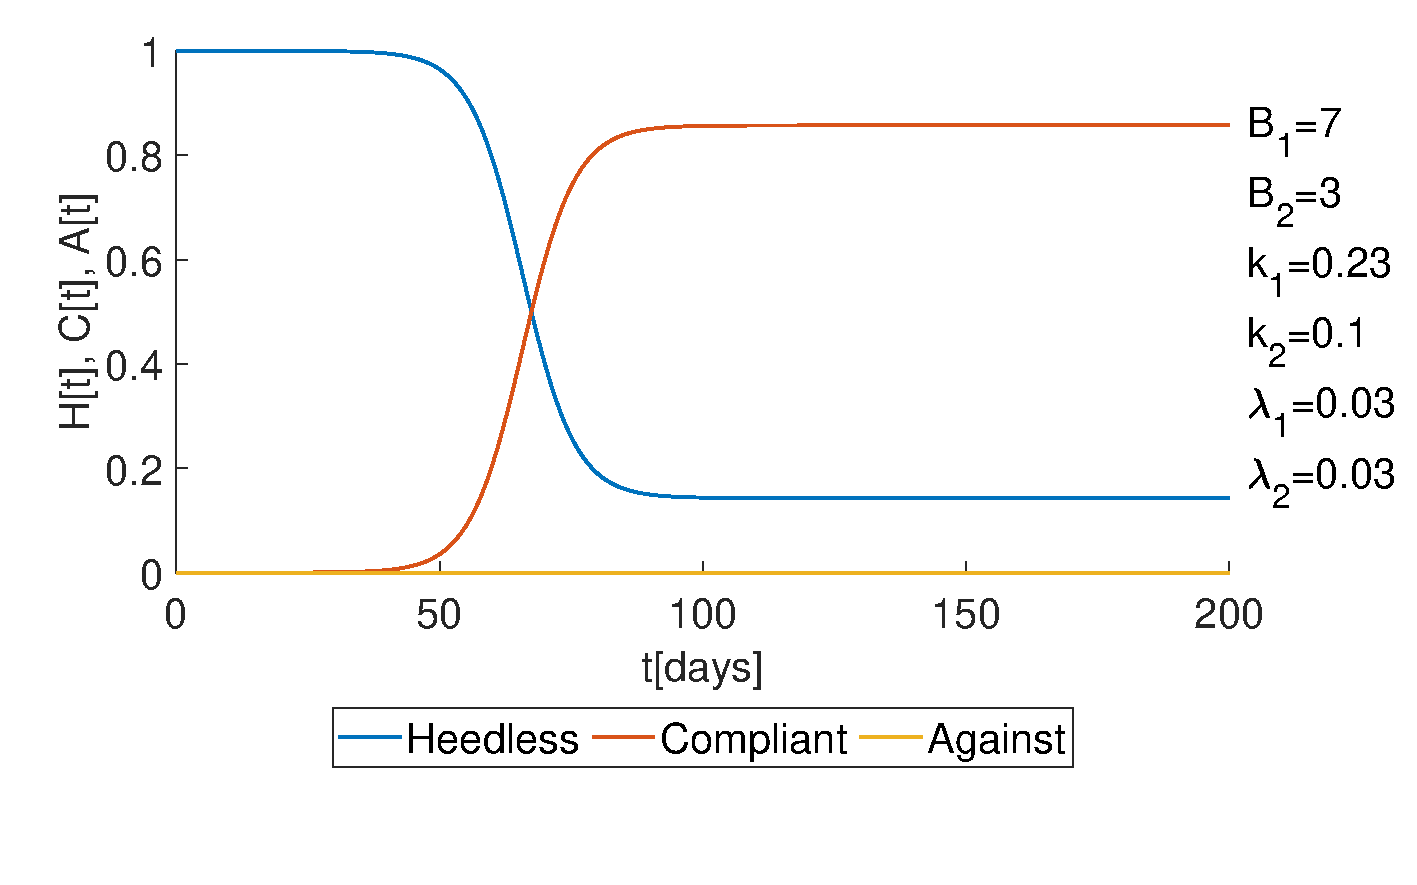
\includegraphics[width=0.48\linewidth]{1_corpo/figure/behavioural_equilibrium/behavior_B1_mag_B2_k1_mag_k2}} \quad
	\subfloat[][\emph{$\mathcal{B}_1, \mathcal{B}_2 >1$ and $\mathcal{B}_1 >  \mathcal{B}_2$, and $\lambda_1 < \lambda_2$.}]
	{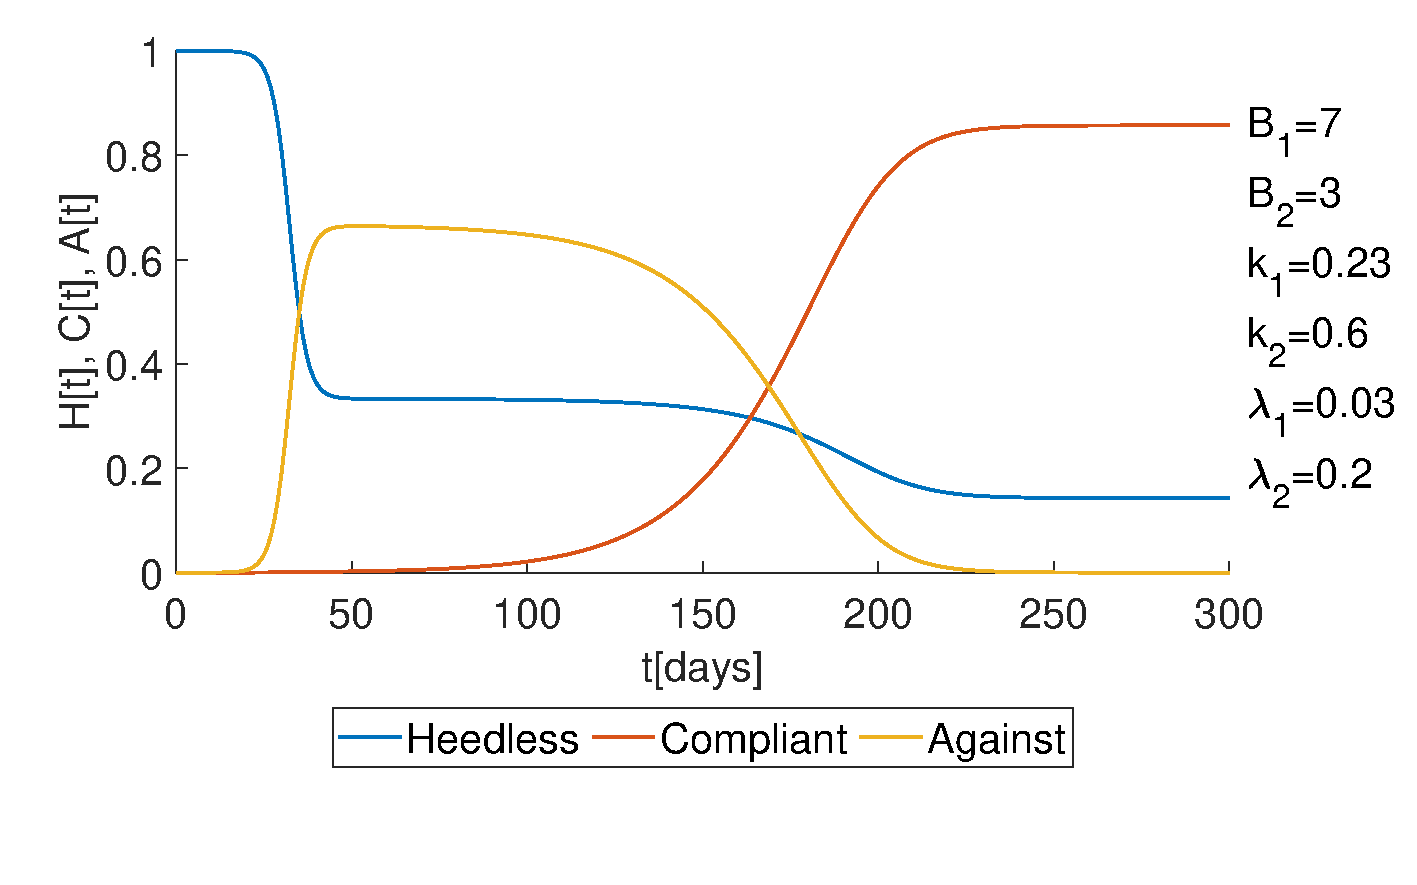
\includegraphics[width=0.48\linewidth]{1_corpo/figure/behavioural_equilibrium/behavior_B1_mag_B2_k2_mag_k1}} \\
		\caption[Behavioral model simulation second]{Behavioral system dynamics: the second two cases (III and IV). In the left panel, the scenario depicts Compliant becoming the dominant group, while Against gradually tends toward zero. In the right panel, with the same value for the conversion number but a higher persuasion rate for Against compared to Compliant, the system converges to the same equilibrium as in the left figure. However, it first goes through a phase where the Against group becomes dominant.}
	\label{fig:model__behavior_sim_2}
\end{figure}

\subsection{Equilibrium and stability analysis}
To enhance our understanding of the system, equilibria are computed and their stability is studied. As observed, the system equilibrium values vary according to parameter values. Specifically, the coefficients were combined to produce two Behavior conversion numbers, $\mathcal{B}_1$ and $\mathcal{B}_2$. One way to identify and visualize the system equilibria for a specific parameter set is through nullclines, used in an autonomous system of differential equations (DE)  to sketch the phase plane of the system. In a system of two DE: 
  
\begin{align}
	\frac{dx}{dt} &= f(x,y) \\
	\frac{dy}{dt} &= g(x,y)
\end{align}

there are two types of nullclines: $x$-nullcline, and $y$-nullcline. The $x$-nullcline is the set of points in the phase plane so that $\frac{dx}{dt} =0$, and graphically can be represented as a set of vectors that go either straight up or down. Instead, the $y$-nullcline is the set of points for which $\frac{dy}{dt} =0$. In these points the vectors are horizontal, going either to the left or to the right.

The original system of three equations, \eqref{eq:behavioural_eq}, has been reduced, to better visualize nullclines in a two-dimensional graph, by using the population conservation assumption: $1 = H + C + A$. By substituting the $A$ term as $A = 1 - H- C$, it is obtained a system of two equations with two unknowns:
\[
\begin{cases}
	\dot{H} = -k_1 H C - k_2 (1-H-C) H + \lambda_1 C + \lambda_2 (1-H-C)\\
	\dot{C} = k_1 H C - \lambda_1 C
\end{cases}
\]
To simplify the readability and use a notation more familiar for plotting,  $H, C$ have been substituted with respectively $x, y$. So, the equations become:
\begin{equation}
\label{eq:system_nullclines}
\begin{cases}
	\dot{x} = -k_1 y x - k_2 (1-y-x) x + \lambda_1 y + \lambda_2 (1-y-x)\\
	\dot{y} = k_1 y x - \lambda_1 y
\end{cases}
\end{equation}
The nullclines can be calculated by imposing $\dot{x} = 0$ and $\dot{y} = 0$. For the first nullcline, with $\dot{x} = 0$,

\begin{equation}\\
\label{eq:x_nullcline}
 y = \frac{x(k_2 - k_2 x + \lambda_2) - \lambda_2}{x(k_2 - k_1)+ \lambda_1- \lambda_2}
\end{equation}
and for the second, with $\dot{y} = 0$,
\[x = \frac{\lambda_1}{k_1} = 1/\mathcal{B}_1 \quad \text{or } y = 0.
\]
%The selection of the correct $\mathcal{B}_i$ to use for the second nullcline depends on the comparison between the two reproductive ratio values. Seeing the result of the simulation, it is understood that the larger value should be chosen, as it represents the behavior that will dominate at equilibrium, while the other behavior will tend toward zero. Only in the case where the $\mathcal{B}_1, \mathcal{B}_2 < 1$ this rule does not hold, because the result of the second nullcline found with the formula is out of the domain of existence (i.e $x > 1$, while the Compliant, $x$ is a value comprised between $[0,1]$.)
The existence condition for the first nullcline can be calculated, imposing that the denominator must not be equal to zero:
\[ x \neq \frac{\lambda_2-\lambda_1}{k_2 - k_1} \]
This value can be in the interval $[0,1]$ only if $\lambda_2>\lambda_1$ and $k_2 > k_1$, or $\lambda_2<\lambda_1$ and $k_2 < k_1$. The second nullcline instead, always exists if $k_1 \neq 0$.

\subsubsection{Equilibria of the system}
The equilibrium value can be computed as the intersection point of the two nullclines, from equation \eqref{eq:x_nullcline}. In fact if $x =\frac{\lambda_1}{k_1}$, then $y = 1 -\frac{\lambda_1}{k_1}$.
Instead if $y = 0$, two values are found: $x = 1$, and $x = \frac{\lambda_2}{k_2}$.
The three equilibria, indicated as $Eq_1, Eq_2 $, and $Eq_3$, are then:
\begin{itemize}
	\item $Eq_1 = (\frac{\lambda_1}{k_1}, 1-\frac{\lambda_1}{k_1})$
	\item $Eq_2 = (1, 0)$
	\item $Eq_3 = (\frac{\lambda_2}{k_2}, 0)$
\end{itemize}

\subsubsection{Equilibria stability analysis}
To assess the local stability of the equilibrium points, the Routh-Hurwitz criterion is applied, requiring the Jacobian matrix of the system evaluated at each equilibrium. The equilibrium is locally stable if:
\begin{itemize}
	\item the trace of the Jacobian is negative: tr($J$)$< 0$
	\item the determinant of the Jacobian is positive: det($J$) $> 0$
\end{itemize}
The Jacobian of the system \eqref{eq:system_nullclines} is
\begin{equation}
	J = \begin{bmatrix}
		-k_1 y -k_2 +k_2 y+2 k_2 x- \lambda_2 & -k_1 x + k_2 x + \lambda_1-\lambda_2 \\
		k_1 y & k_1 x - \lambda_1
	\end{bmatrix}
\end{equation}
The trace of $J$ is
\begin{equation}
	\text{tr}(J) = -k_1 y -k_2 +k_2y + 2 k_2 x - \lambda_2 -\lambda_1 +k_1 x
\end{equation}
Its determinant is instead
\begin{equation}
	\text{det}(J) = k_2 \lambda_1 + \lambda_1 \lambda_2 + 2 k_1 k_2 x^2 - k_1 k_2 x - k_1 \lambda_2 x - 2\cdot k_2 \lambda_1 x + k_1 \lambda_2 y - k_2 \lambda_1 y
\end{equation}

For each equilibrium point, stability conditions can be expressed as relationship between the coefficients $k_1, k_2$, and $\lambda_1, \lambda_2$.\\

%%%%%%%%%%%%%%%%%%%%%%%%%%%%%%%%%%%%%%%%%%%%%%%%%%%%%%%
\noindent\textbf{Stability of equilibrium $Eq_1$=$(\frac{\lambda_1}{k_1}, 1-\frac{\lambda_1}{k_1})$.} The trace tr$(J(Eq_1)) = - k_1 + \frac{\lambda_1}{k_1}(k_1+k_2) - \lambda_2$ is  less than zero, if $-k_1 + \frac{\lambda_1}{k_1}( k_1 + k_2) - \lambda_2 < 0$. From this we obtained the relation:
\[\frac{\lambda_1}{k_1} < \frac{k_1 + \lambda_2}{k_1 + k_2} \]
Instead, the determinant is det$(J(Eq_1)) = k_1 \lambda_2 - \lambda_1 \lambda_2 -k_2 \lambda_1 + k_2 \frac{\lambda_1^2}{k_1}$. The determinant is greater than zero if
 \[ k_1^2 \lambda_2+ k_2 \lambda_1^2 - k_1 k_2 \lambda_1 -k_1 \lambda_1 \lambda_2 > 0.\]
  Then, $k_1 \lambda_2(k_1 -\lambda_1) - k_2 \lambda_1 (k_1 - \lambda_1) > 0$, and so $(k_1 - \lambda_1)(k_1 \lambda_2 - k_2 \lambda_1) > 0$. The condition is satisfied when both factors are greater or less than zero. Considering both factors negative results in a condition $\mathcal{B}_1 < 1$, which has no biological meaning because the equilibrium resulting from this condition would have a negative value.

The conditions $\mathcal{B}_1 > 1$ and $\mathcal{B}_1 > \mathcal{B}_2$ satisfy the determinant condition, but are also compatible with the the trace condition.
To understand why, let us consider $\mathcal{B}_1 > 1$, which implies $\frac{\lambda_1}{k_1} < 1$. This ensure that the trace wil be negative if the following inequality holds:
\[\frac{k_1 + \lambda_2}{k_1 + k_2} > 1.\] 
Simplifying this expression gives $k_1 + \lambda_2 > k_1 + k_2$, which reduces further to  $\lambda_2 > k_2$. This directly implies $\mathcal{B}_2 < 1$. Thus, the trace condition is automatically satisfied by the two conditions already imposed by the determinant, making it redundant.
In conclusion, equilibrium $Eq_1$ is locally stable if $\mathcal{B}_1 > 1$, and $\mathcal{B}_1 > \mathcal{B}_2$.
\\ 
 
%%%%%%%%%%%%%%%%%%%%%%%%%%%%%%%%%%%%%%%%%%%%%%%%%%%%%%%
\noindent\textbf{Stability of equilibrium $Eq_2=(1,0)$.} Calculating the Jacobian determinant at this point yields the expression det$(J(Eq_2))= - k_2 \lambda_1 + \lambda_1 \lambda_2 + k_1 k_2 - k_1 \lambda_2$. By grouping terms and analyzing the inequality necessary to satisfy the Routh-Hurwitz criterion, this simplifies to $k_1 (k_2 - \lambda_2) - \lambda_1(k_2 - \lambda_2) > 0$, which further reduces to $(k_1 - \lambda_1) (k_2 - \lambda_2) >0$.
This inequality is satisfied if both terms in the product are either positive or negative:
\begin{itemize}
	\item Case $I:$ $k_1 > \lambda_1$, and $k_2 > \lambda_2$
	\item Case $II:$ $k_1 < \lambda_1$, and $k_2 < \lambda_2$
\end{itemize}
Evaluating the trace at this point, the result is tr$(J(Eq_2)) = k_2 - \lambda_2 - \lambda_1 + k_1 < 0 $. Rearranging terms gives the condition $k_1 + k_2 < \lambda_1 + \lambda_2$, which is true only under Case $II$ identified above. 
Thus, it can be concluded that equilibrium point $B$ is locally stable only if $\frac{k_1}{\lambda_1} <1$, and  $\frac{k_2}{\lambda_2} <1$, which correspond to $\mathcal{B}_1 < 1$, and $\mathcal{B}_2 <1$.\\

%%%%%%%%%%%%%%%%%%%%%%%%%%%%%%%%%%%%%%%%%%%%%%%%%%%%%%%
\noindent\textbf{Stability of equilibrium $Eq_3=(\frac{\lambda_2}{k_2},0)$.} The determinant at this point is given by det$(J(Eq_3)) = k_2 \lambda_1 - \lambda_1 \lambda_2 + k_1 \frac{\lambda_2^2}{k_2} - k_1 \lambda_2 > 0 $. Also here, rearranging terms simplifies the inequality to: $k_2 [\lambda_1 -\lambda_1 \frac{\lambda_2}{k_2} + k_1 \frac{\lambda_2^2}{k_2^2} - k_1 \frac{\lambda_2^2}{k_2}] >0$, $ k_2 [\lambda_1 ( 1 -  \frac{\lambda_2}{k_2}) - k_1 \frac{\lambda_2}{k_2} (1 - \frac{\lambda_2}{k_2})] >0$, which further reduces to:

\[
 k_2 \left[\left(\lambda_1 - k_1 \frac{\lambda_2}{k_2}\right)\left(1 - \frac{\lambda_2}{k_2}\right)\right] >0
\]
To satisfy the inequality both terms inside the parentisi must have the same sign, as in the previous point $Eq_2$:
\begin{itemize}
	\item Case $I:$ $\frac{k_2}{\lambda_2} > \frac{k_1}{\lambda_1} $, and $k_2 > \lambda_2$
 	\item Case $II:$ $\frac{k_2}{\lambda_2} < \frac{k_1}{\lambda_1} $, and $k_2 < \lambda_2$
\end{itemize}

The trace value is given by:
\[
\text{tr}(J(Eq_3)) = -k_2 + k_2 \frac{\lambda_2}{k_2} + k_1 \frac{\lambda_2}{k_2} - \lambda_1 < 0,
\]
leading to the inequality:
\[
\frac{\lambda_2}{k_2} (k_1 + k_2) < k_2 + \lambda_1,
\]
which simplifies to:
\[
\frac{\lambda_2}{k_2} < \frac{k_2 + \lambda_1}{k_1 + k_2}.
\]

Only by choosing Case I, we ensure that the trace inequality is satisfied. If \(k_2 > \lambda_2\), the ratio \(\frac{\lambda_2}{k_2}\) is less than one. Thus, if the right-hand side of the inequality is larger than one, the trace condition holds. Specifically:
\[
\frac{k_2 + \lambda_1}{k_1 + k_2} > 1 \implies k_2 + \lambda_1 > k_1 + k_2 \implies \lambda_1 > k_1.
\]

While the trace condition is satisfied when \(\mathcal{B}_1 < 1\), it is redundant, analogous to the trace condition found for equilibrium \(Eq_1\). Therefore, it can be concluded that equilibrium \(Eq_3\) is stable if \(\mathcal{B}_2 > \mathcal{B}_1\) and \(\mathcal{B}_2 > 1\).

 
\subsection{Equilibrium simulations}

Based on the equilibrium analysis, we now understand how the model behaves with various parameter values. To confirm these results, nullcline plots for the four previously simulated cases are generated, and the different scenarios are examined. First, it is important to describe what can be visualized in the nullcline plot. The blue curve is the expression found solving the x-nullcline, and the vertical line in the plot correspond to the point of discontinuity of this expression, as discussed before. The green line is instead the y-nullcline, composed of a vertical and a horizontal line, representing the two possible solutions. In purple the three equilibria points are visualized. If stable, they are marked with a diamond, will unstable with a circle.  
The values of coefficients used in the five cases are:
\begin{center}
 \begin{tabular}{|c|c|c|c|c|}
 	\hline
 	& $B_1$ & $\lambda_1 \,[d^{-1}]$ & $B_2$ & $\lambda_2 \, [d^{-1}]$ \\
 	\hline
 	case I & 0.89 & 1/30 & 0.45 & 1/40 \\
 	\hline
 	case II & 8.5 & 1/25 & 8.5 & 1/30 \\
 	\hline
 	case III & 7 & 1/30 & 3 & 1/30 \\
 	\hline
 	case IV & 7 & 1/30 & 3 & 1/5 \\
 	\hline
 	case V & 0.6 & 1/20 & 4& 1/30 \\  
 	\hline
 \end{tabular}
\end{center}
Variables $k_1$ and $k_2$ are derived using the expression $\mathcal{B}_i = k_i/\lambda_i$, where $i = 1, 2$.\\
%%%%%%%%%%%%%%%%%%

\noindent\textbf{I case: }$\mathcal{B}_1, \mathcal{B}_2 <1$, $\mathcal{B}_1 >  \mathcal{B}_2$, and $\lambda_1 > \lambda_2$. \\
If both the Conversion numbers are less than one, there is only one equilibrium in the phase plane, where both Compliant and Against are zero.

In the Figure \ref{fig:r1r2less1dyn}a, the nullcline plot shows an intersection between the two nullclines only at the point $(1,0)$. Under this condition, the only equilibrium is at $H = 1$, with both $A$ and $C$ equal to zero. Using the notation from the system equation \eqref{eq:system_nullclines}, this corresponds to $x = 1$ and $y = 0$. Calculating the trace and determinant of the Jacobian at this point and with parameters value


yields tr$J(1,0) = -\frac{209}{12000}$ and det$J = \frac{121}{2400000}$. Thus, the equilibrium is locally asymptotically stable, as it satisfies the Routh-Hurwitz condition.\\

\begin{figure}[ht]
	\centering
	\subfloat[][\emph{$\mathcal{B}_1, \mathcal{B}_2 <1$, $\mathcal{B}_1 >  \mathcal{B}_2$, and $\lambda_1 > \lambda_2$. Point B, corresponding to $Eq_2$ is the stable equilibrium}]
	{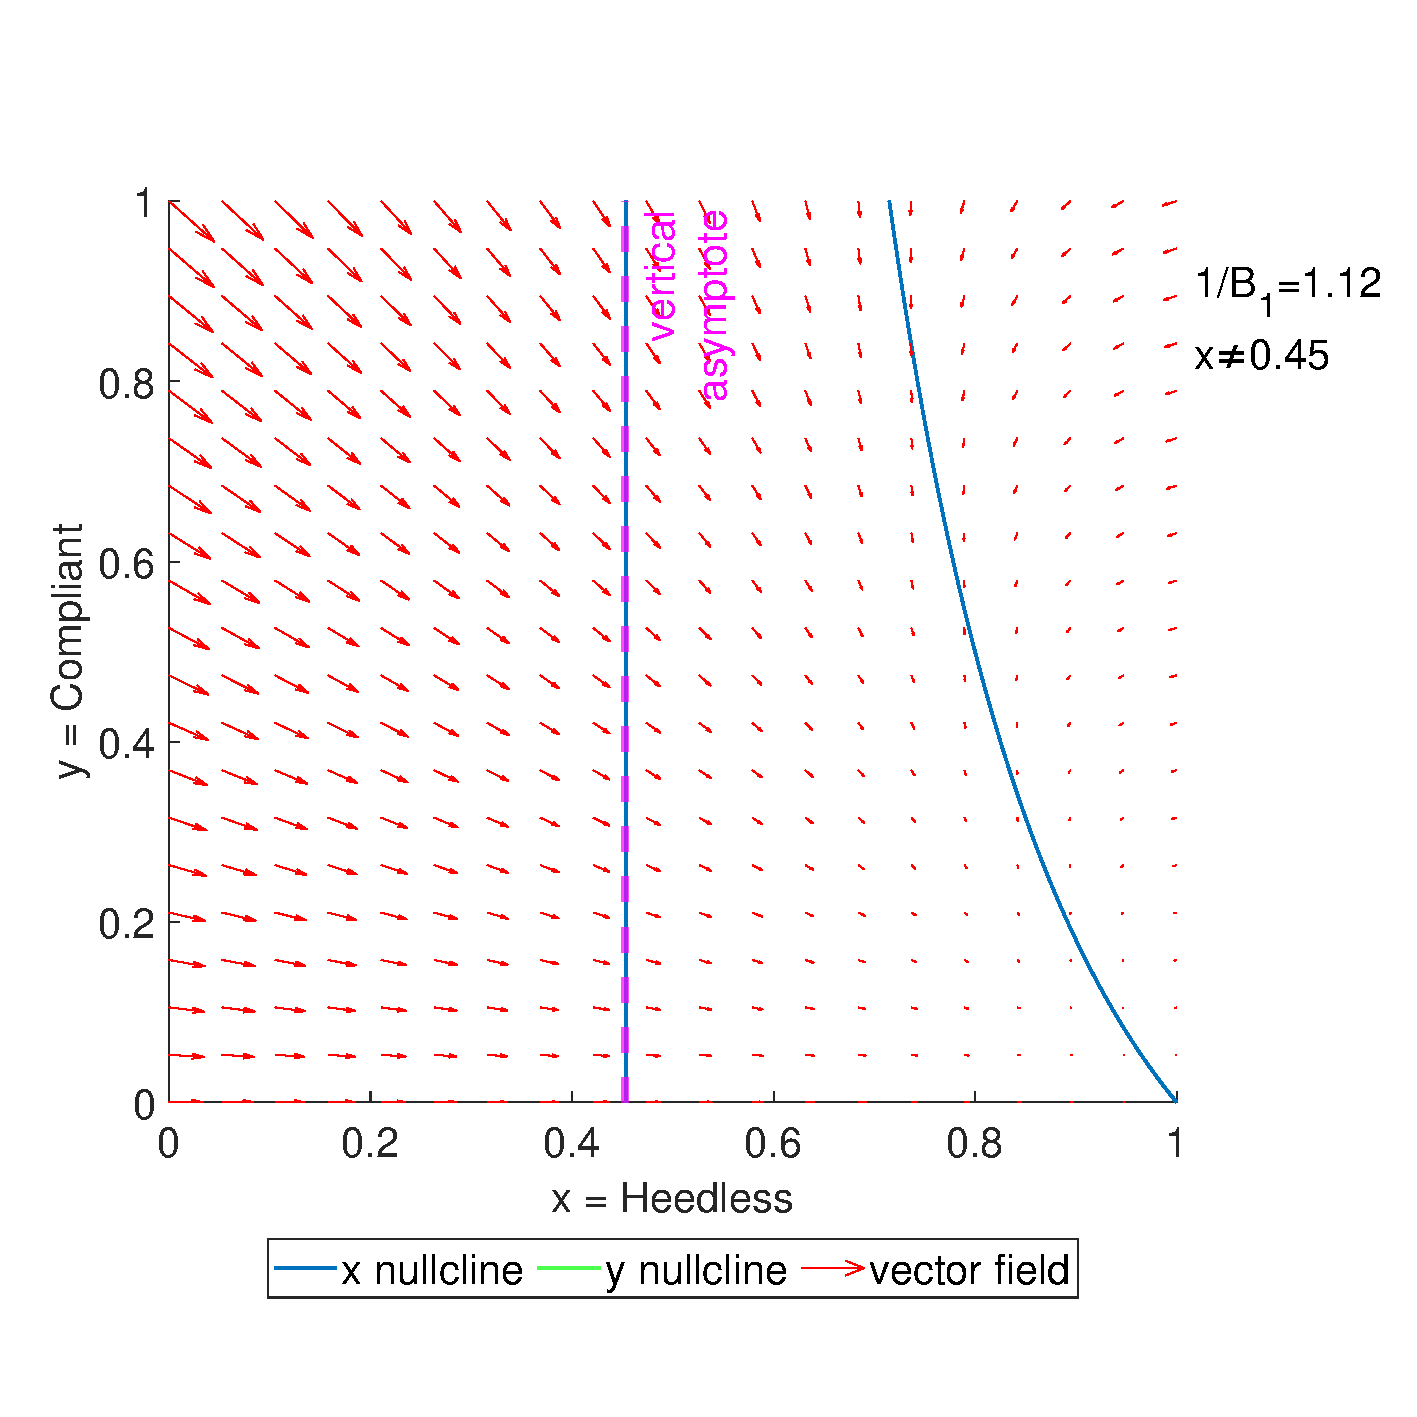
\includegraphics[width=0.48\linewidth]{1_corpo/figure/behavioural_equilibrium/Pr_nullcline_B1_B2_less_1}} \quad
	\subfloat[][\emph{$\mathcal{B}_1, \mathcal{B}_2 >1$, $\mathcal{B}_1 =  \mathcal{B}_2$, and $\lambda_1 < \lambda_2$.} There is not a stable equilibrium in this case.]
	{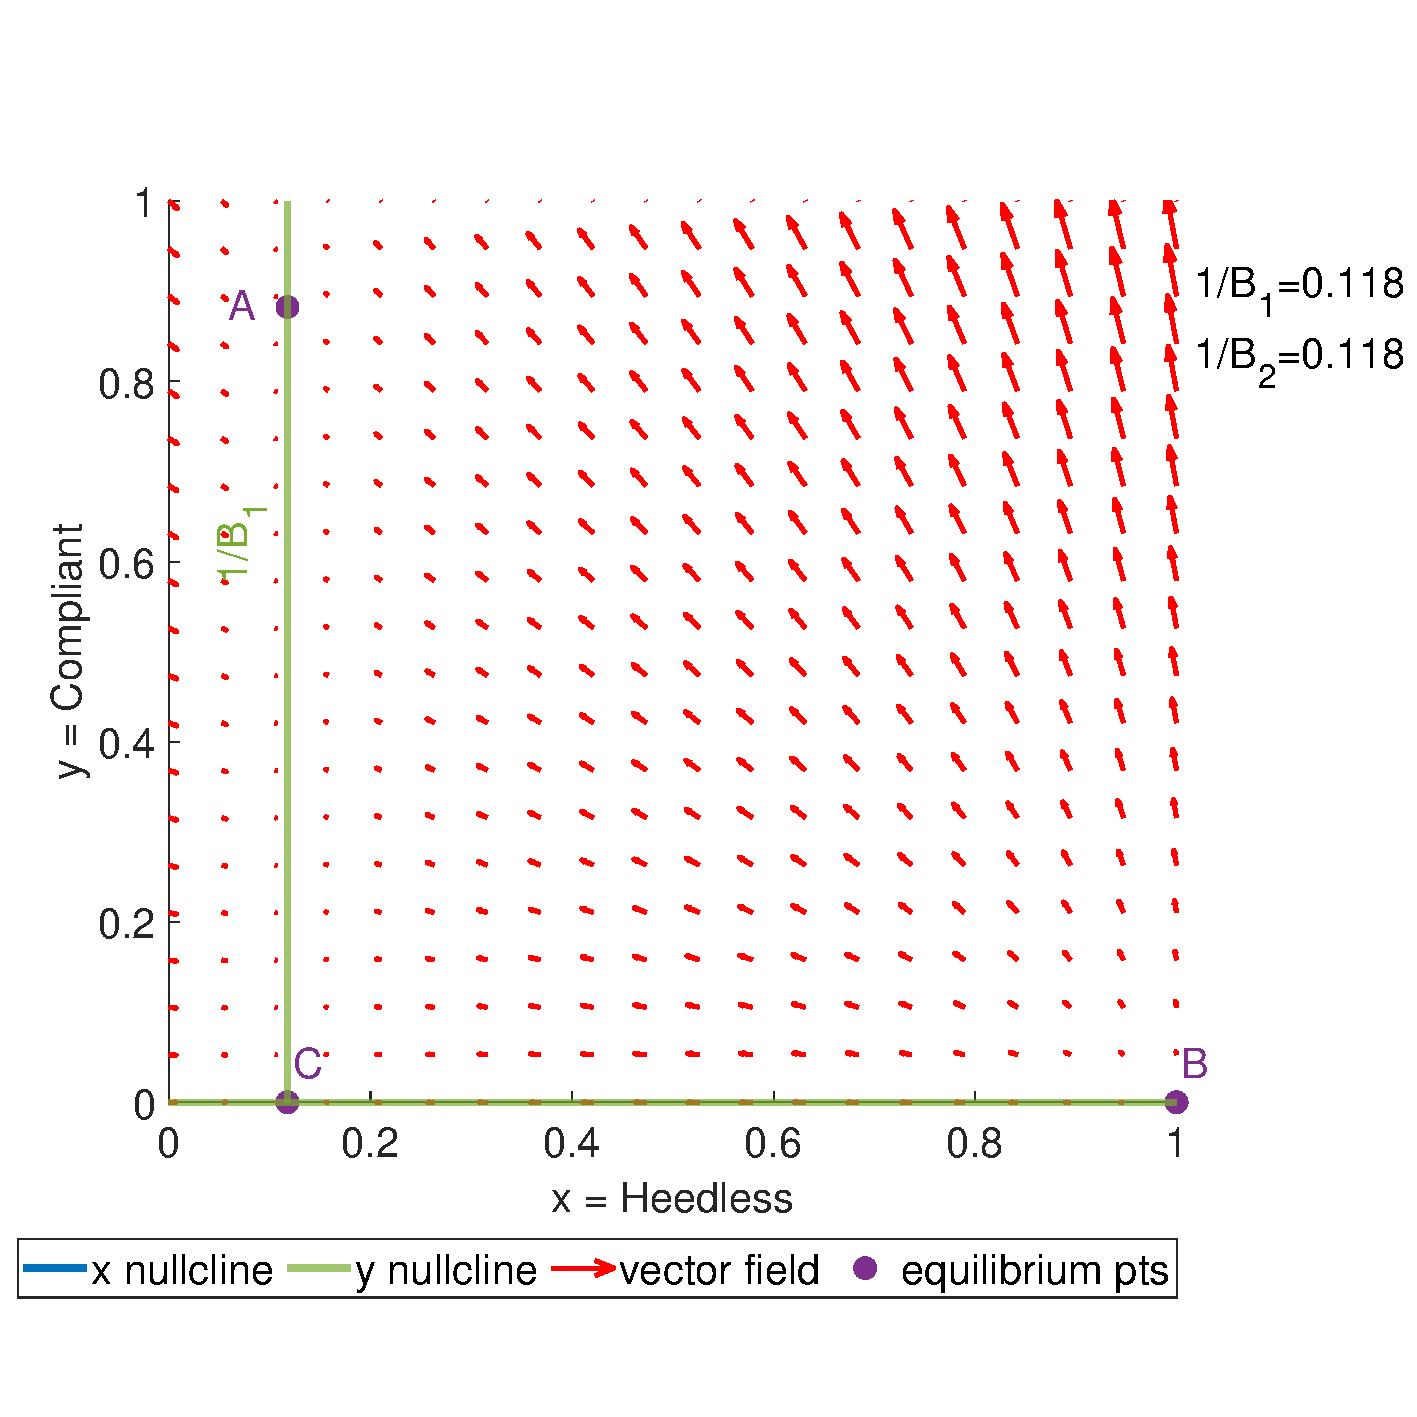
\includegraphics[width=0.48\linewidth]{1_corpo/figure/behavioural_equilibrium/Pr_nullcline_B1_B2_equal}} \\
	\caption[Nullclines first figure]{Nullclines plots of the first two situations analyzed: In (a) the case in which both $\mathcal{B}_1, \mathcal{B}_21$ are less than one. (b) is the phase plane representation when $\mathcal{B}_1 = \mathcal{B}_2 <1$.  }
	\label{fig:r1r2less1dyn}
\end{figure}
%%%%%%%%%%%%%%%%%%

\noindent\textbf{II case: } $\mathcal{B}_1, \mathcal{B}_2 >1$, $\mathcal{B}_1 =  \mathcal{B}_2$, and $\lambda_1 < \lambda_2$.\\
This second situation is the most complex to analyze. Due to the equal value of the two influence processes, the asymptotic value of the state variables cannot be determined solely by the previously established relations but also depends on the initial conditions.

The Heedless density at the equilibrium can still be determined as previously discussed, and the same value is obtained for both $x = \lambda_1/k_1$ and $x = \lambda_2/k_2$. Thus, the final equilibrium value of $x$ is $\bar{x} = 0.12$.
Also the equilibrium $(1,0)$ is possible, but is certainly unstable with the parameter value considered in this case. As it can be seen from the system evolution in Figure \ref{fig:model__behavior_sim_1}, and nullcline plots of Figure \ref{fig:r1r2less1dyn}, at the equilibrium $\bar{x}$, the Against and Compliant  sums up to $ y + z = 1 - \bar{x}$ part, where $y$ represent Compliant and $z$ Against. The ratio between $A$ and $C$ depends on the initial conditions.
%\begin{figure}[h]
%	\centering
%	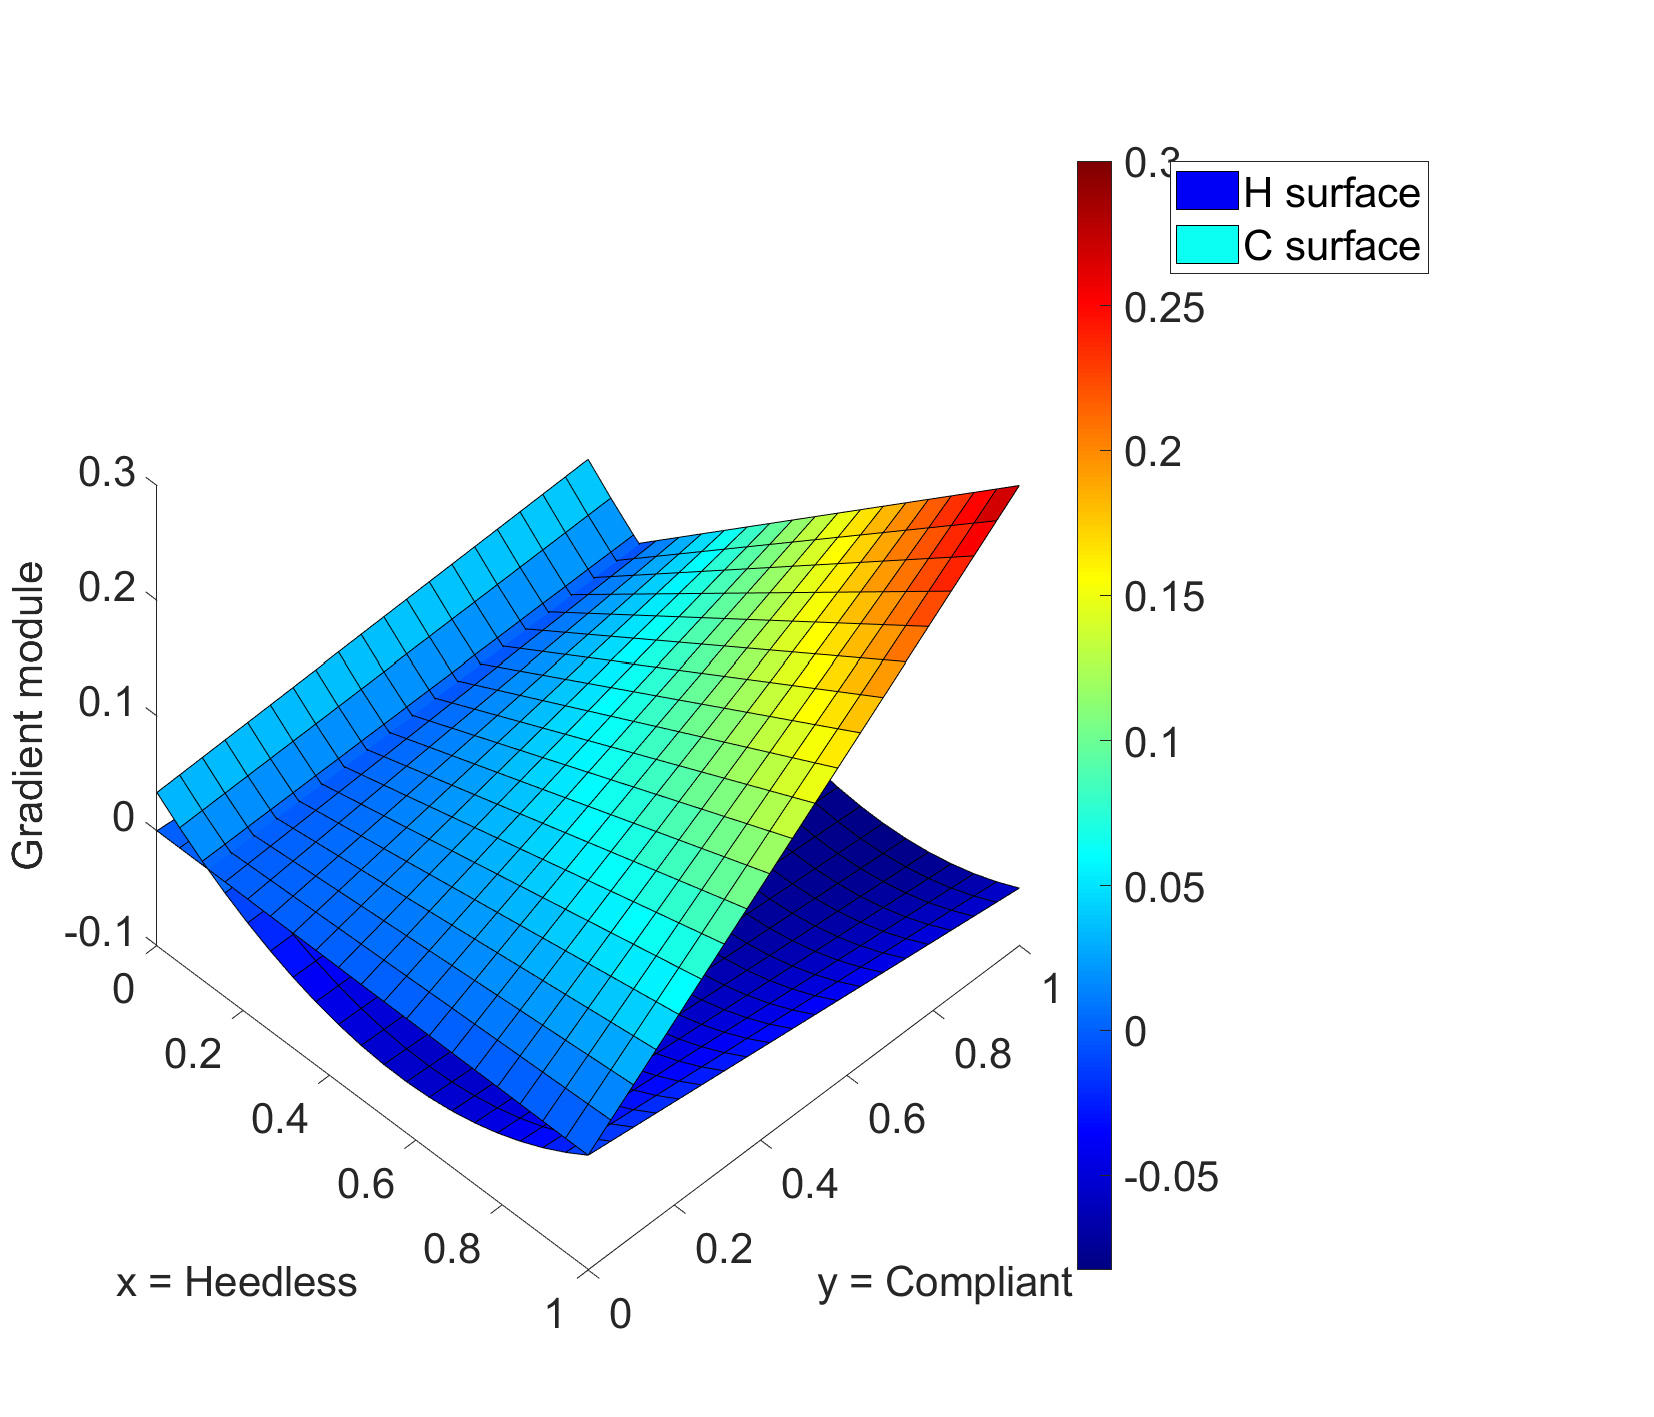
\includegraphics[width=0.7\linewidth]{1_corpo/figure/behavioural_equilibrium/Surface_nullcline_B1_equal_B2}
%	\caption[Surface nullcline]{The nullcline functions represented as surfaces in a tridimensional space.}
%	\label{fig:surfacenullclineb1equalb2}
%\end{figure}
Applying the Routh-Hurwitz criterion does not yield information on this equilibrium because the Jacobian determinant equals zero. An explanation for this is that, given the equilibrium alignment of points $A$ and $C$ and the equality of their conversion numbers, the influxes and outfluxes between the Compliant and Against compartments balance. Consequently, the system evolution is influenced by the initial numbers of Compliant and Against individuals, and once the system reaches the equilibrium value of Heedless, it remains in this configuration. \\
%Observing the 3D plot in Figure \ref{fig:surfacenullclineb1equalb2} of the complete system, with surfaces for $H$ and $C$, one can visualize a slope where an imaginary inertia-free ball would roll until it settles at the $1/\mathcal{B}_1 = 1/\mathcal{B}_2$  value.\\
%%%%%%%%%%%%%%%%%%%%%%%%%%%%


\noindent\textbf{III case:} $\mathcal{B}_1, \mathcal{B}_2 >1$, $\mathcal{B}_1 >  \mathcal{B}_2$, and $\lambda_1 = \lambda_2$. \\
In this scenario, as shown in Figure \ref{fig:nullcline_B1_mag_B2}, there is an intersection between the two nullclines, at the point 0 . The equilibrium has coordinates $x_{Eq_1} = \lambda_1/k_1$ and $y_{Eq_1} = 1 - \lambda_1/k_1 $, derived by solving the nullcline expressions as previously described. $trJ(\bar{x},\bar{y}) = -23/105$, and $detJ(\bar{x},\bar{y}) = 2/525$, so the equilibrium is locally asymptotically stable and the solution converges to it regardless of the initial conditions.\\
%%%%%%%%%%%%%%%%%%%%%%%%%%%%

 
\begin{figure}[ht]
	\centering
	\subfloat[][\emph{ $\mathcal{B}_1, \mathcal{B}_2 >1$, $\mathcal{B}_1 >  \mathcal{B}_2$, and $\lambda_1 = \lambda_2$.} The point A, ($Eq_1$) is the stable equilibrium.]
	{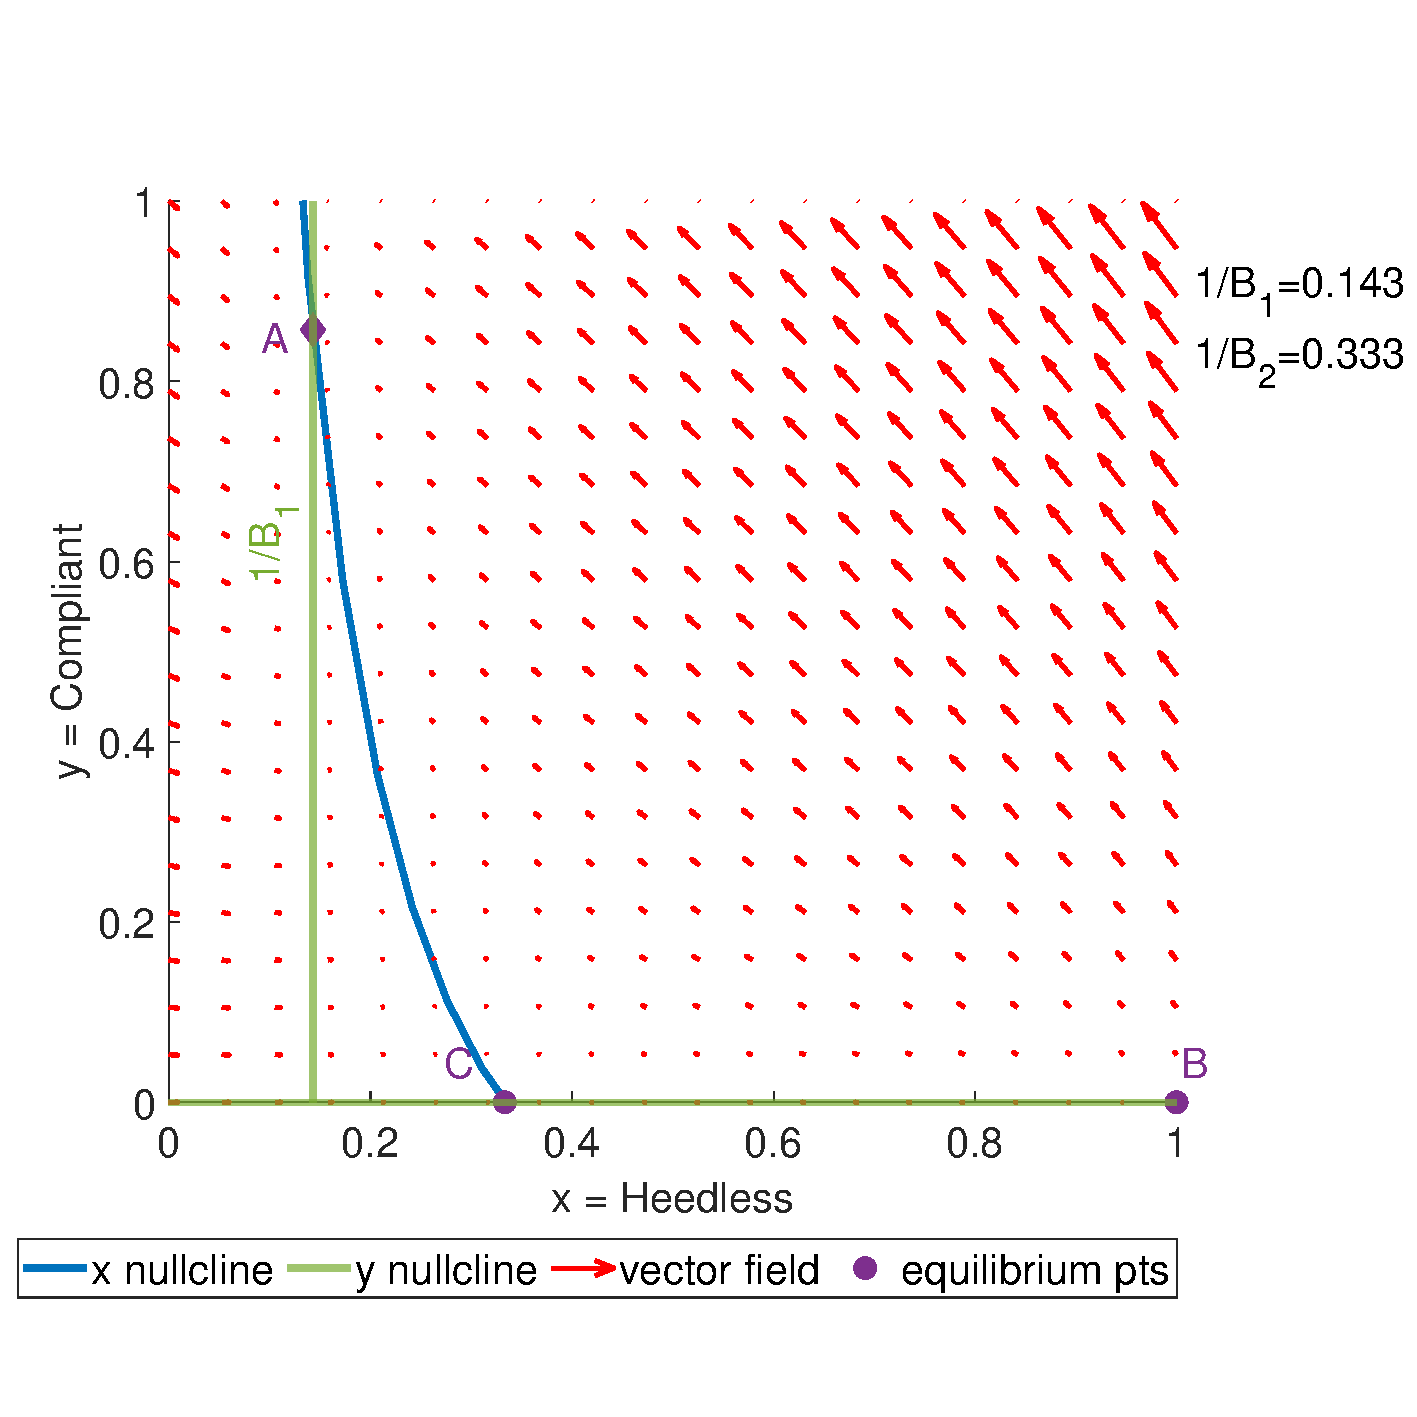
\includegraphics[width=0.48\linewidth]{1_corpo/figure/behavioural_equilibrium/Pr_nullcline_B1_mag_B2}} \quad
	\subfloat[][\emph{ $\mathcal{B}_1<1, \mathcal{B}_2 >1$ and $\mathcal{B}_2 >  \mathcal{B}_1$.} Point C, corresponding to $Eq_3$ is the stable equilibirum.]
	{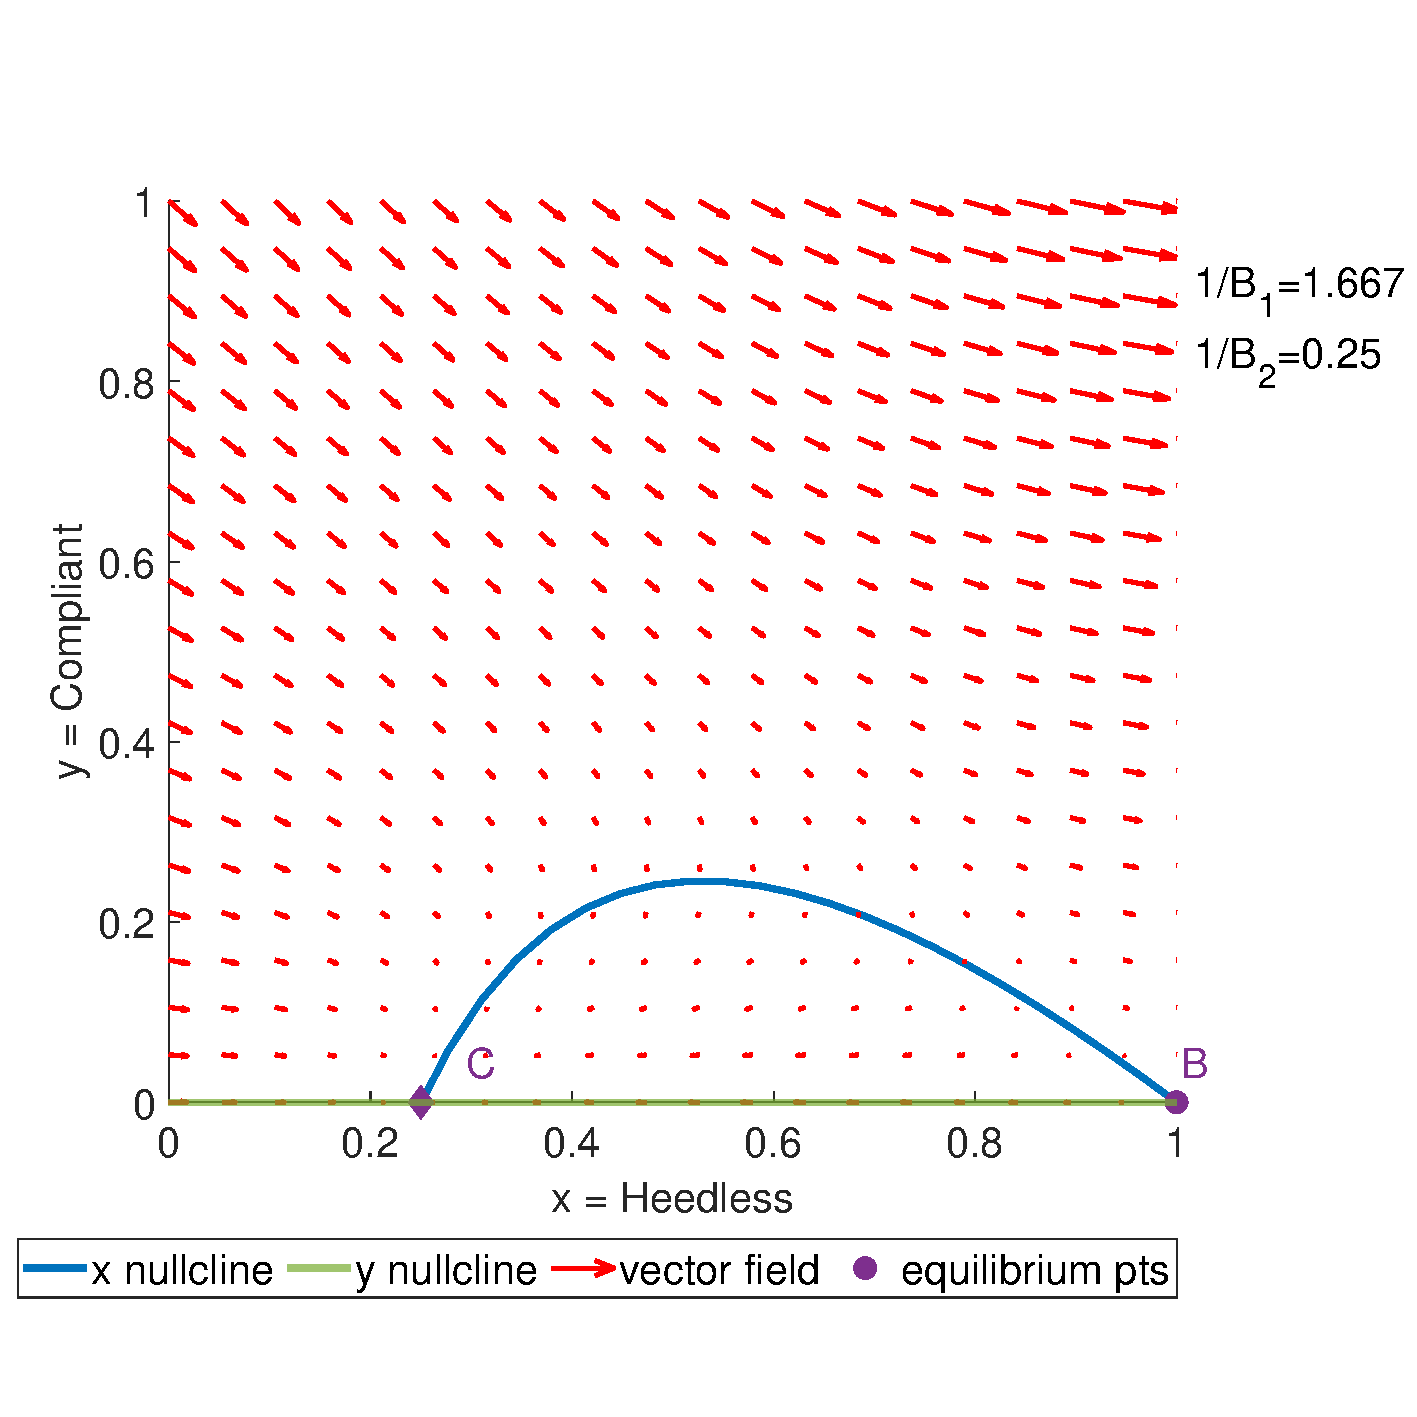
\includegraphics[width=0.48\linewidth]{1_corpo/figure/behavioural_equilibrium/Pr_nullcline_B1_less_B2}} \\
	\caption[Nullclines second figure]{Nullclines plots of the third and fifth cases: in (a) $\mathcal{B}_1 >  \mathcal{B}_2$ and the phase plane arrows point to A equilibrium. In (b), where $\mathcal{B}_1 <  \mathcal{B}_2$, the stable equilibrium is in point B, where there is no Compliant.}
	\label{fig:nullcline_B1_mag_B2}
\end{figure}

\begin{figure}[ht]
	\centering
	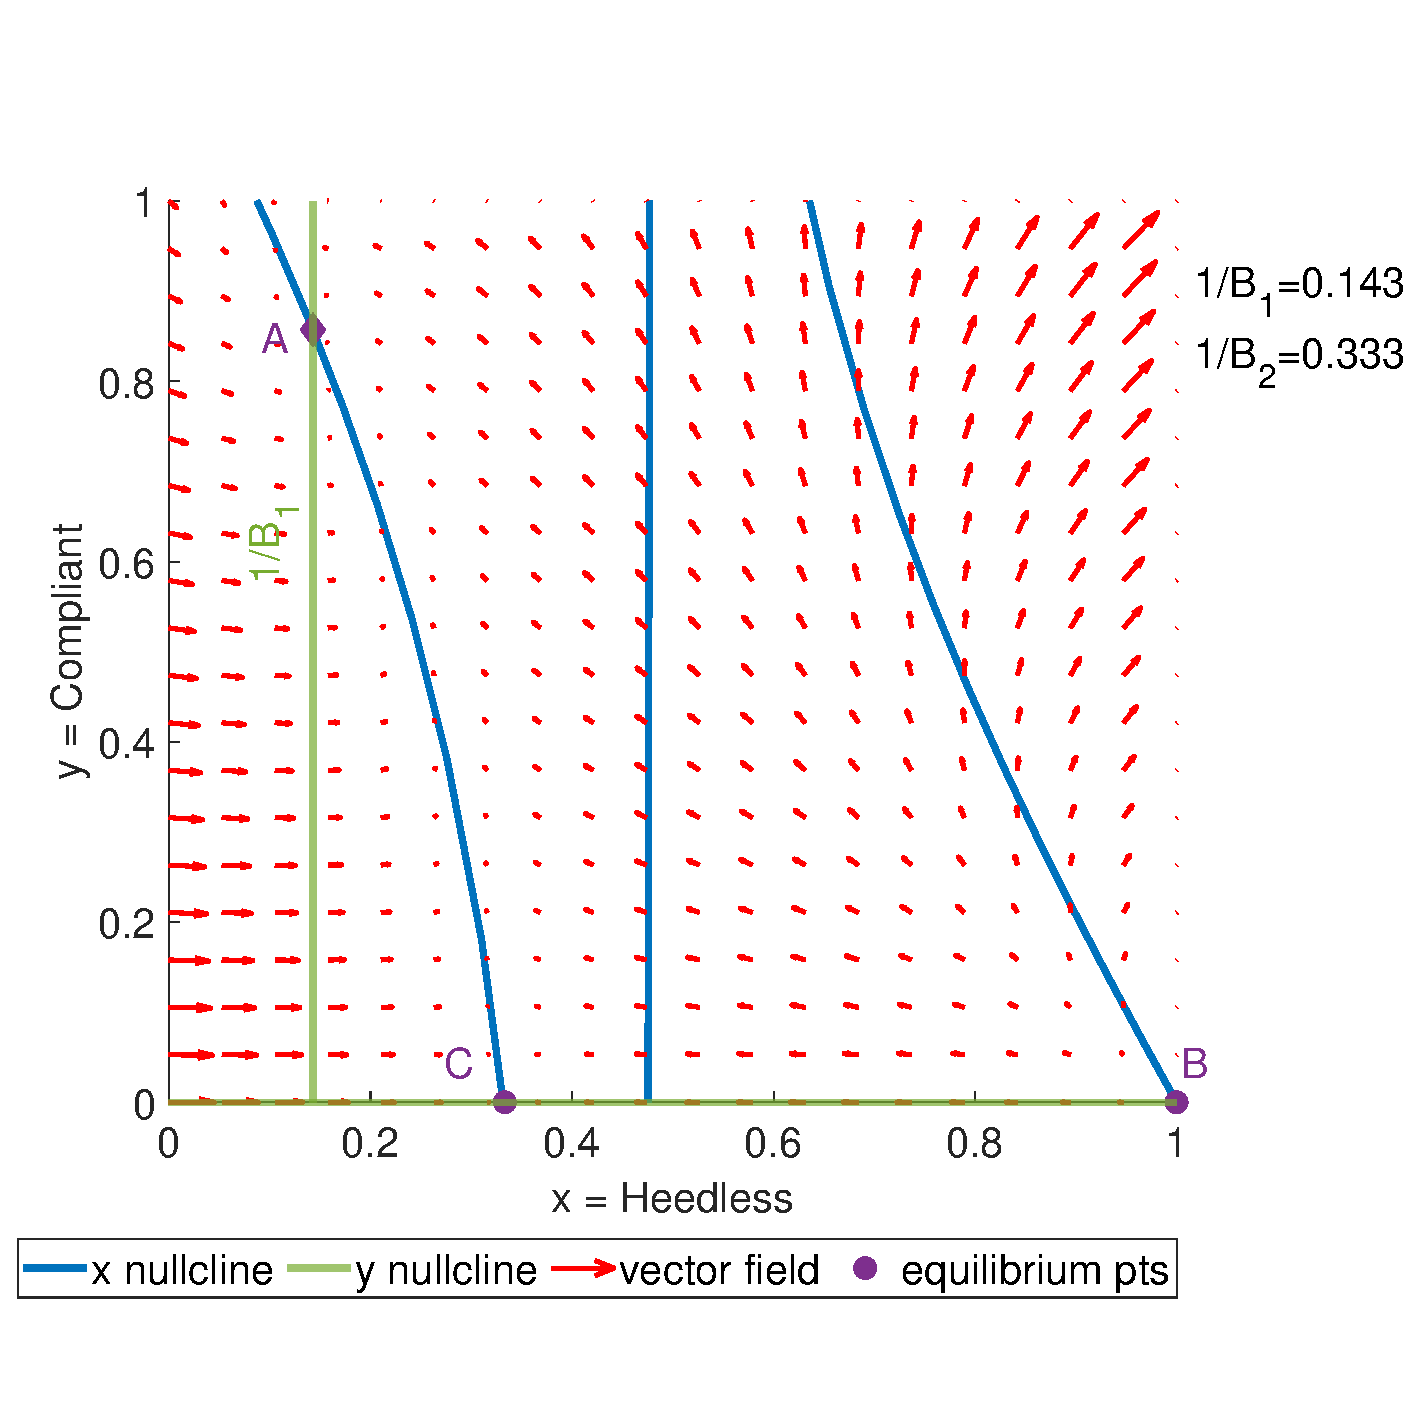
\includegraphics[width=0.48\linewidth]{1_corpo/figure/behavioural_equilibrium/Pr_nullcline_B1_mag_B2_lambda2_mag}
	\caption[Nullcline fourth case]{IV case of nullcline simulation. A point (corresponding to $Eq_1)$ is the locally stable equilibrium.}
	\label{fig:prnullclineb1_mag_b2_lambda}
\end{figure}

\noindent\textbf{IV case: } $\mathcal{B}_1, \mathcal{B}_2 >1$ and $\mathcal{B}_1 >  \mathcal{B}_2$, and $\lambda_1 < \lambda_2$. \\
\label{par:behav_4_case}
In this situation, the equilibrium has the same value, as in III case, and also the stability condition are verified. However, the nullcline plot is very different as shown in Figure \ref{fig:prnullclineb1_mag_b2_lambda}. 
In fact, looking at the model simulation in Figure \ref{fig:model__behavior_sim_2}, the system initially evolves to what seems as a first equilibrium, corresponding to $x_{Eq_3} = \lambda_2/k_2$, $y_{Eq_3} = 0$. However, this equilibrium is unstable (as verified with the Routh-Hurwitz criterion),and so the model continues its evolution until it reaches the locally stable equilibrium.\\ 


\noindent\textbf{V case: $\mathcal{B}_1 < 1$ $\mathcal{B}_2 >1$, $\mathcal{B}_1 <  \mathcal{B}_2$.}\\
The system's evolution shows opposite behavior compared to the third case, with the Compliant, tending to zero at equilibrium. The right panel of Figure \ref{fig:nullcline_B1_mag_B2}, shows two intersections in the phase plane at points $Eq_2$ and $Eq_3$. At both points, $y=0$, but only point $Eq_3$ is locally stable, as it satisfies the Routh-Hurwitz conditions. The equilibrium point is calculated as $x_{E_q3}= \lambda_2/k_2$ and $y_{E_q3} = 0$. 


\subsection{Behavioural model: numerical experiments}
To better understand all possible scenarios emerging from the behavioral model, a set of simulations is conducted. Four vectors are defined, one for each model parameter, and a separate simulation is performed for each parameter combination. During each simulation, the parameter values remain constant. The variation range for each parameter is as follows:
\begin{itemize}
	\item $k_1$ between $0.1$ and $0.99$
	\item $k_2$ between $0.1$ and $0.99$
	\item $\lambda_1$ between $1/2$ and $1/40$ $d^{-1}$
	\item $k_1$ between $1/2$ and $1/40$ $d^{-1}$
\end{itemize}
varied with twenty equally spaced steps.
The resulting $\mathcal{B}_1, \mathcal{B}_2$ have a range spanning between $0.5$, and $29.7$.
These ranges are chosen based on the assumption that the "fatigue" rate realistically spans between two and forty days, a range supported by prior research, such as the study in \cite{Kwasnicka_2016}. For the behavior persuasion rate ($k_1$, $k_2$), both low and high values for transition rates are included. We observe the dynamics across all states, recording key metrics for each simulation, such as the final compartment values, peak values, and the time of peak occurrence. Additionally, for generating the sensitivity plots, the Conversion number derived from the coefficient combinations in equation \eqref{eq:behave_rate} are applied. 

\subsubsection{Heat map: asymptotic state values}


\begin{figure}[ht]
	\centering
	\subfloat[][\emph{ Compliant }]
	{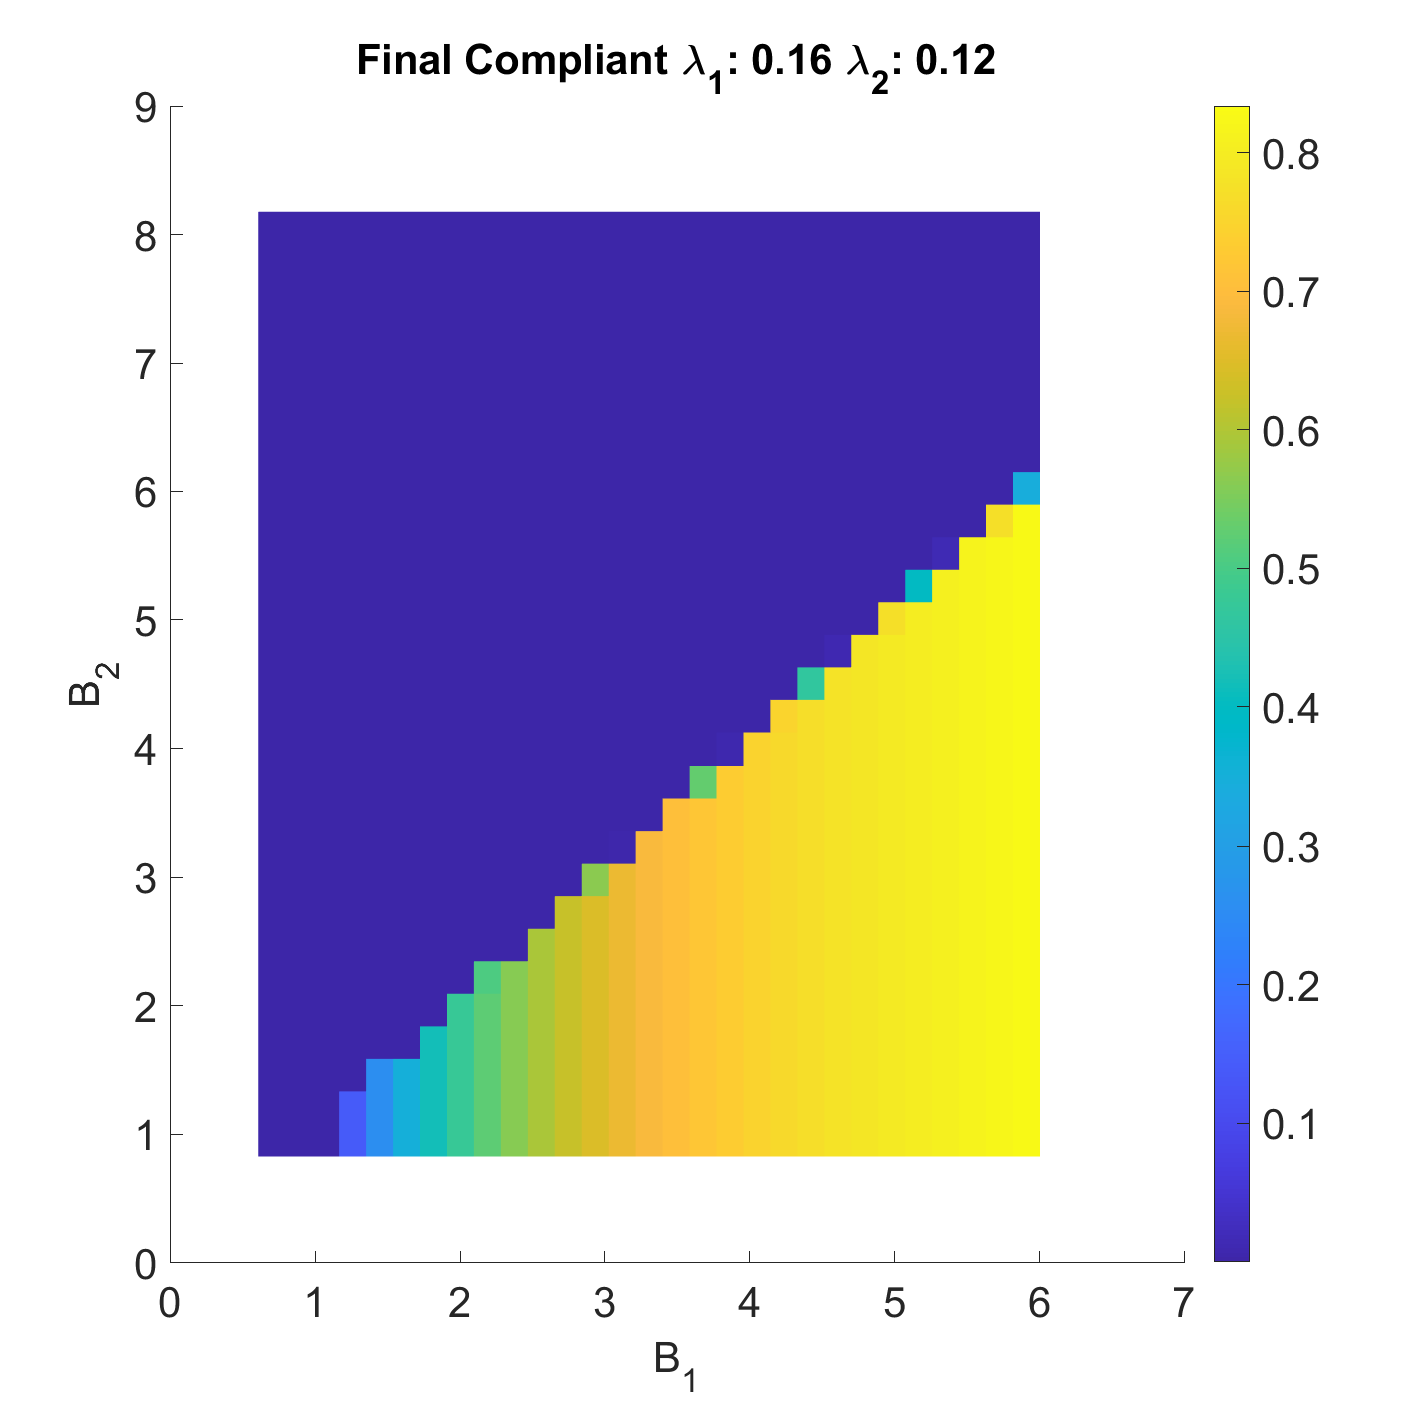
\includegraphics[width=.48\textwidth]{1_corpo/figure/behavioural_equilibrium/Final_Compliant_heat_map}} \quad
	\subfloat[][\emph{ Against }]
	{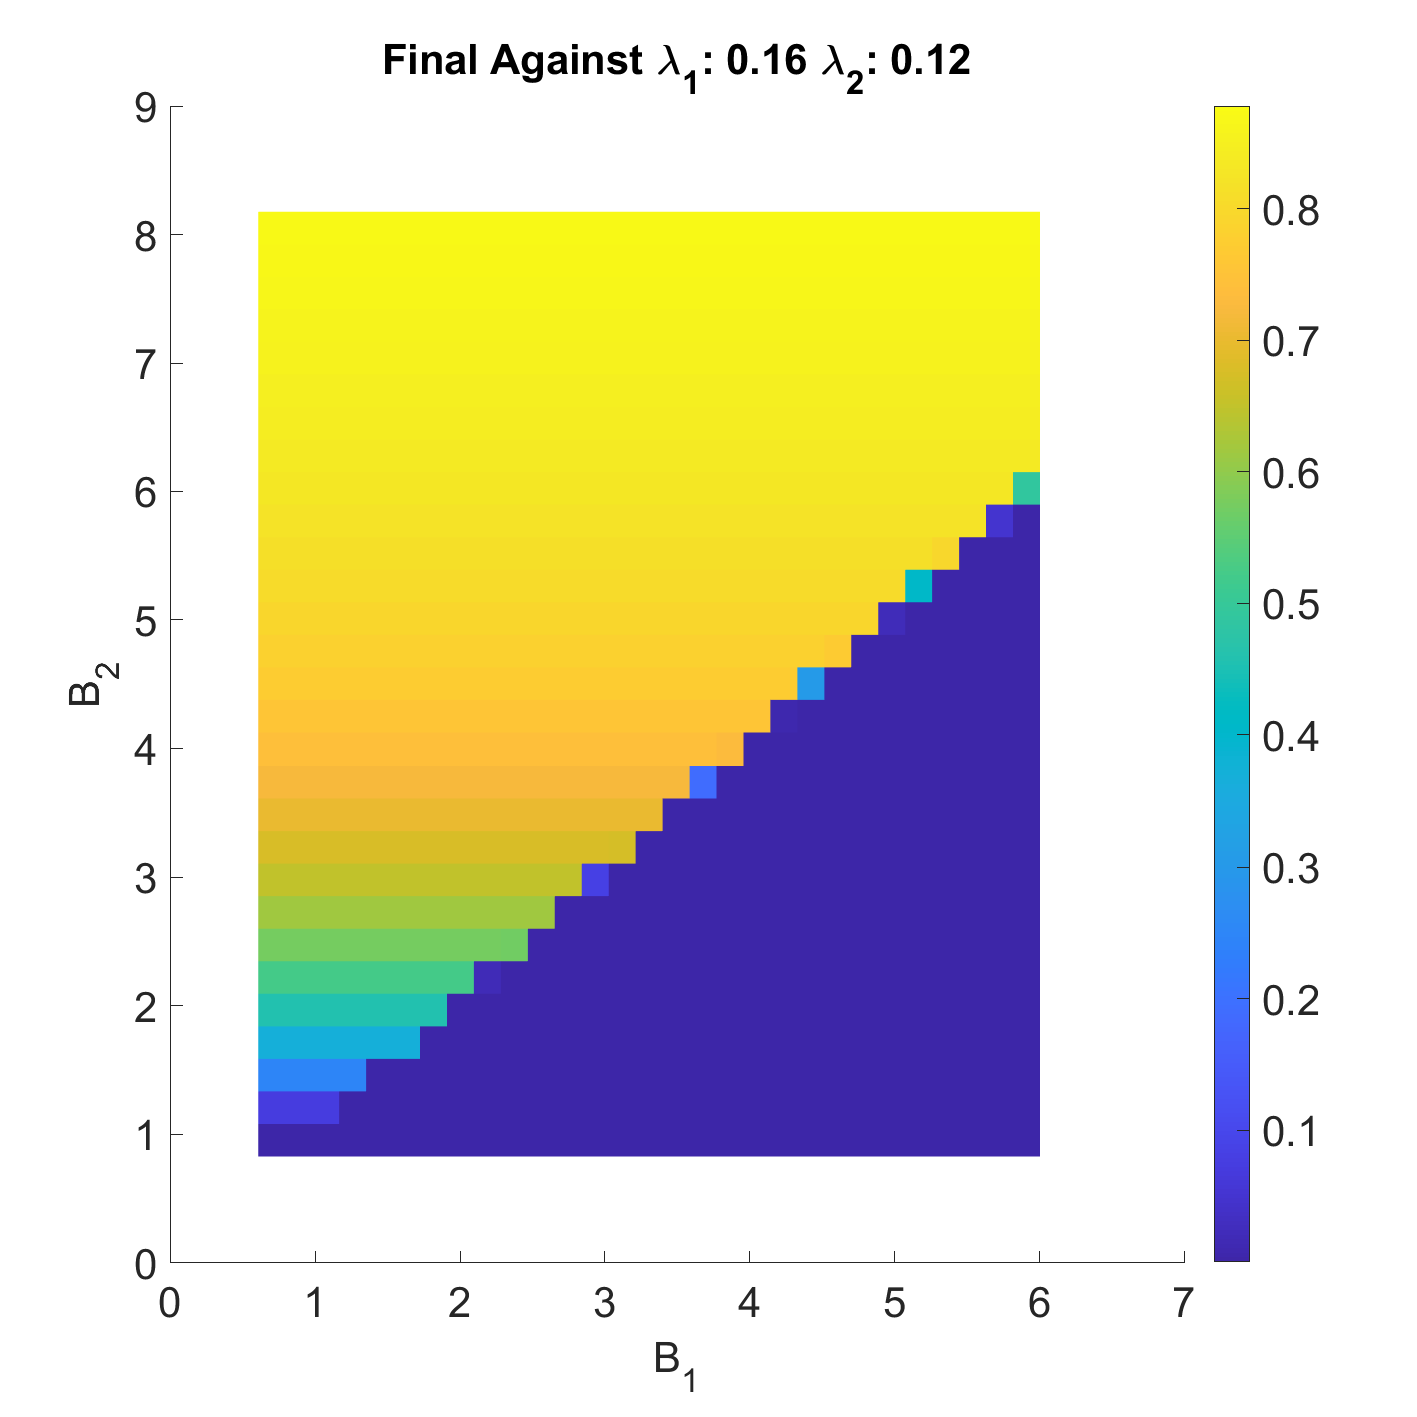
\includegraphics[width=.48\textwidth]{1_corpo/figure/behavioural_equilibrium/Final_Against_heat_map}} \\
	\subfloat[][\emph{ Heedless }]
	{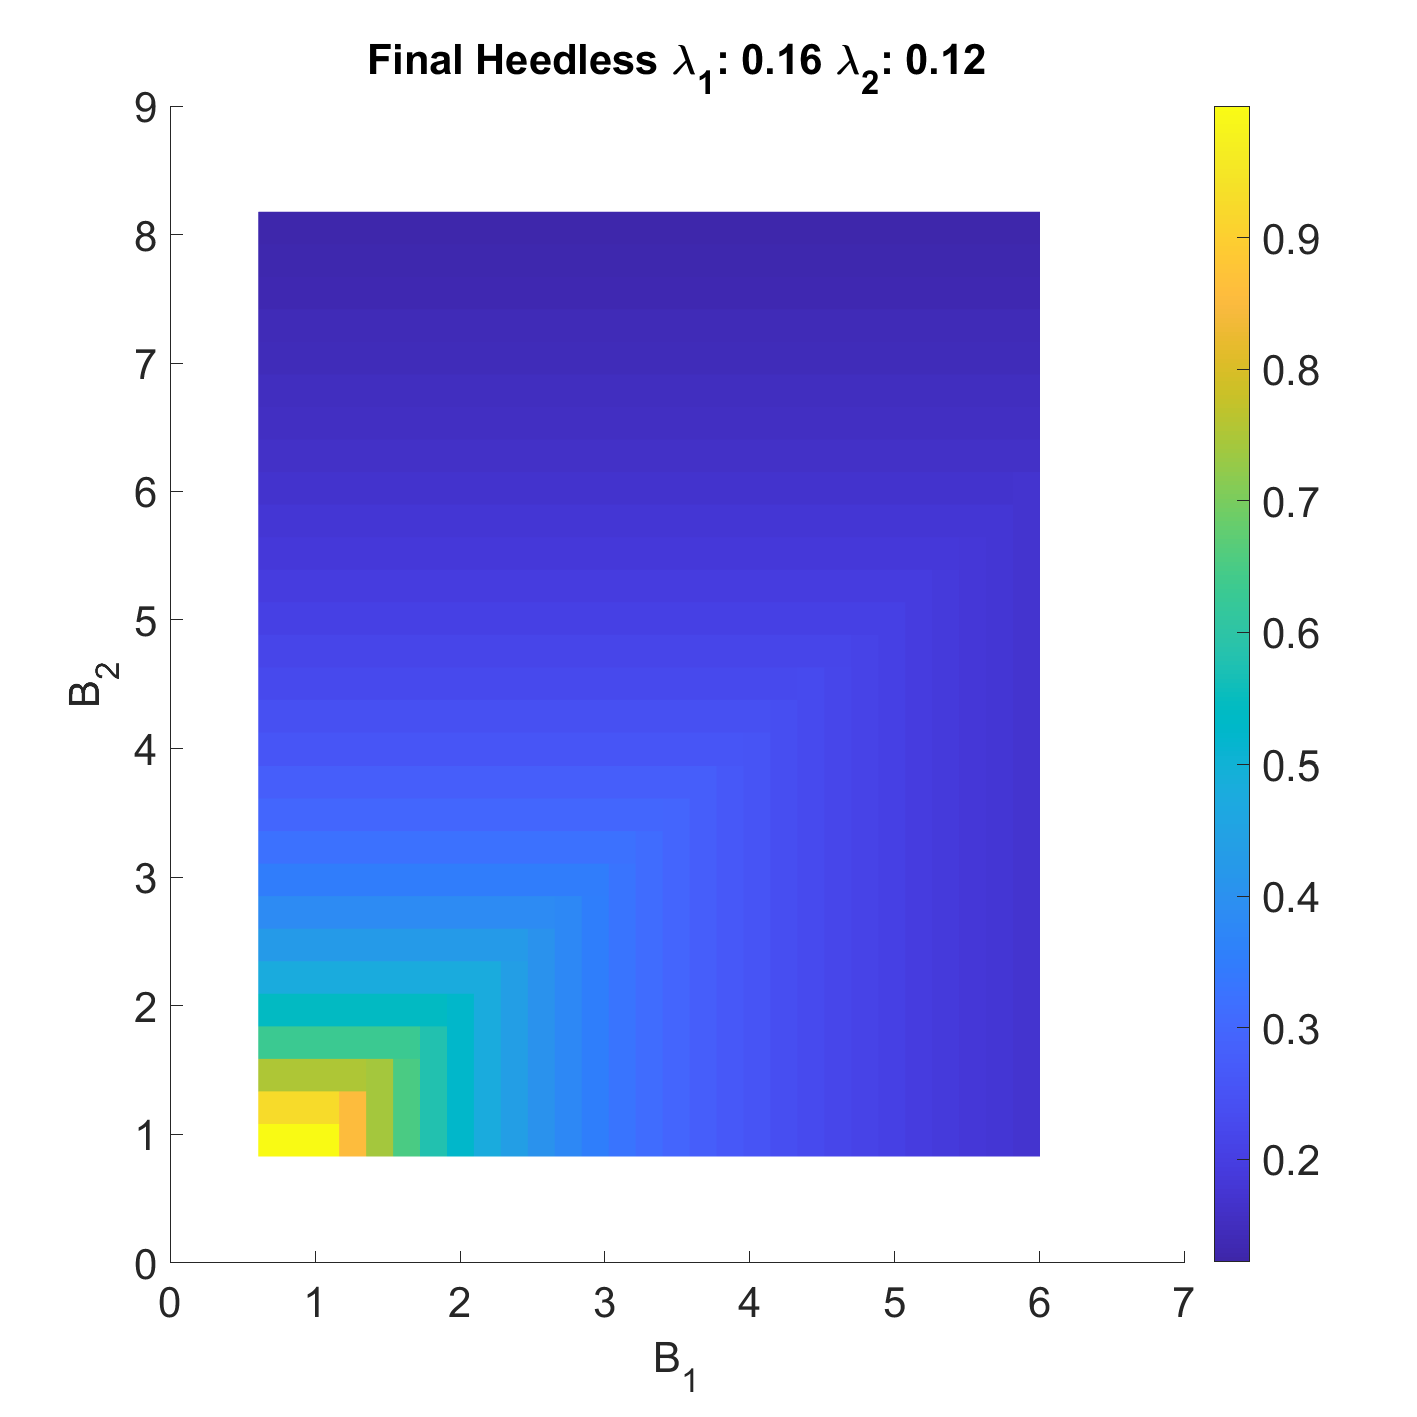
\includegraphics[width=.48\textwidth]{1_corpo/figure/behavioural_equilibrium/Final_Heedless_heat_map}}
	\caption[Final Behavioural variables]{The asymptotic value reached at the equilibrium by the variables in the behavioral model.}
	\label{fig:subfig_sensitivity_behavioural}
\end{figure}
Figure \ref{fig:subfig_sensitivity_behavioural} shows heat maps of the final value reached by the various variables, for varying $\mathcal{B}_1$ and $\mathcal{B}_2$.
The threshold effect observed in the stability analysis performed earlier is clearly visible. While one of the reproduction ratios becomes larger than the other, the population is composed of the dominant group from either $C$ and $A$ and plus a number of Heedless individuals. The larger are $\mathcal{B}_1$ and $\mathcal{B}_2$, and the more distant from 1 is their ratio, the  smaller is the equilibrium fraction of the Heedless. Considering Figure \ref{fig:subfig_sensitivity_behavioural}a, until $\mathcal{B}_1 > \mathcal{B}_2$ Compliant behavior is dominant. Then, in the area of the heat map where the conversion number $\mathcal{B}_1, \,\mathcal{B}_2$ are similar (which correspond to the diagonal clearly visible) the two groups have similar density. Finally, when $\mathcal{B}_1$ becomes smaller than $\mathcal{B}_2$, the Compliant abruptly tend to zero. This threshold effect can also be observed in Figure \ref{fig:subfig_sensitivity_behavioural_r1}.

\begin{figure}[ht]
	\centering
	\subfloat[][\emph{ Compliant }]
	{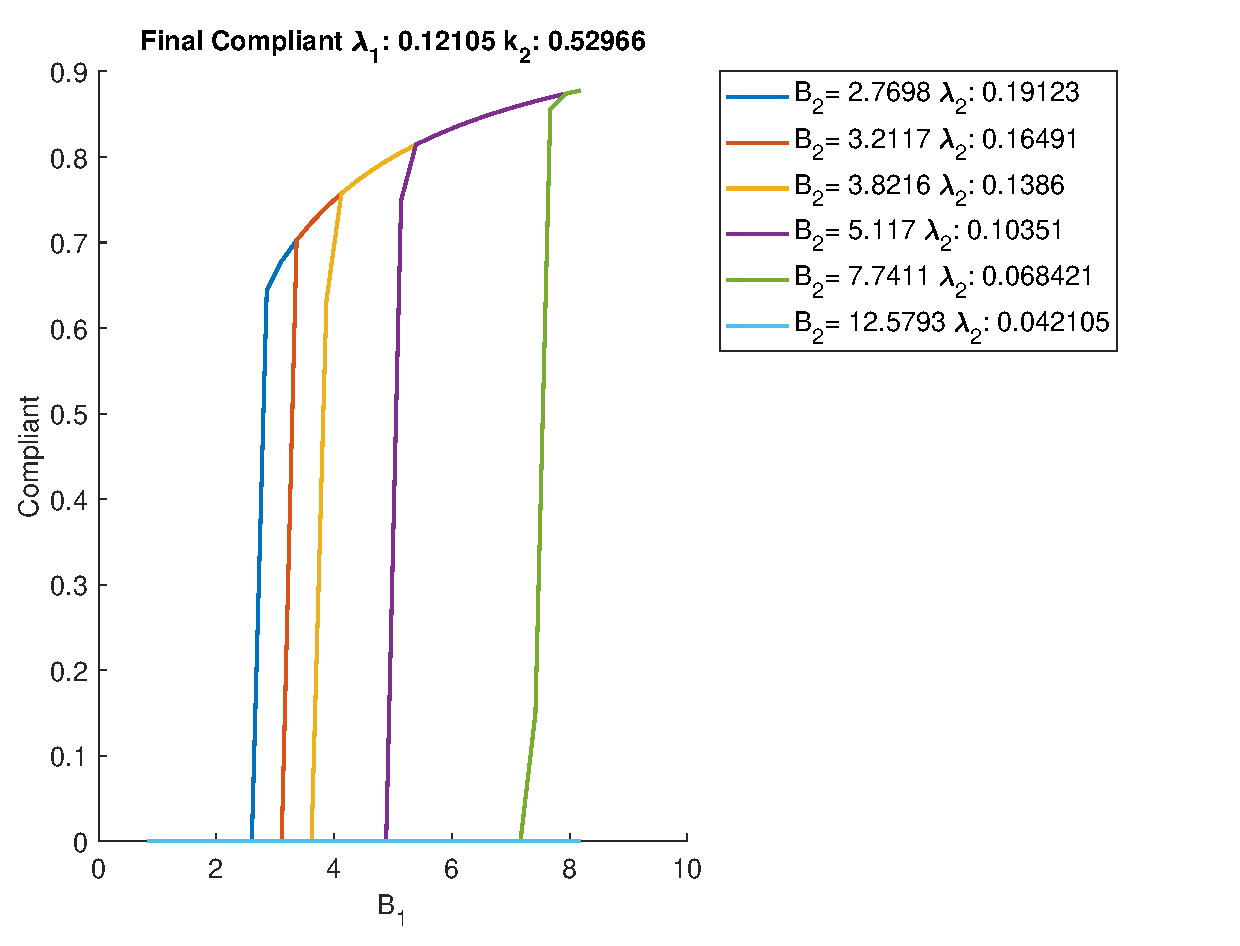
\includegraphics[width=.48\textwidth]{1_corpo/figure/behavioural_equilibrium/final_compliant_B1}} \quad
	\subfloat[][\emph{ Against }]
	{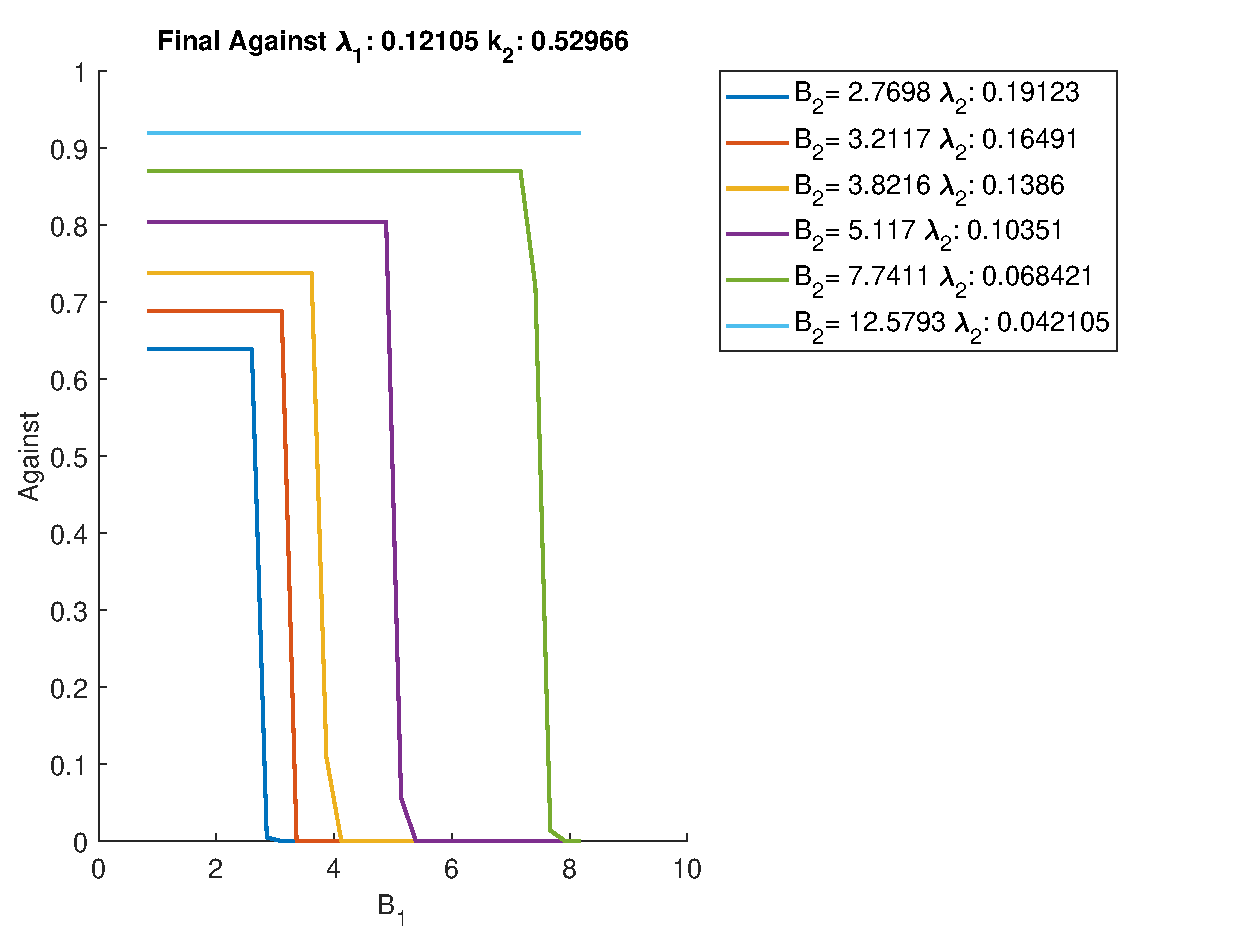
\includegraphics[width=.48\textwidth]{1_corpo/figure/behavioural_equilibrium/final_against_B1}} \\
	\subfloat[][\emph{ Heedless }]
	{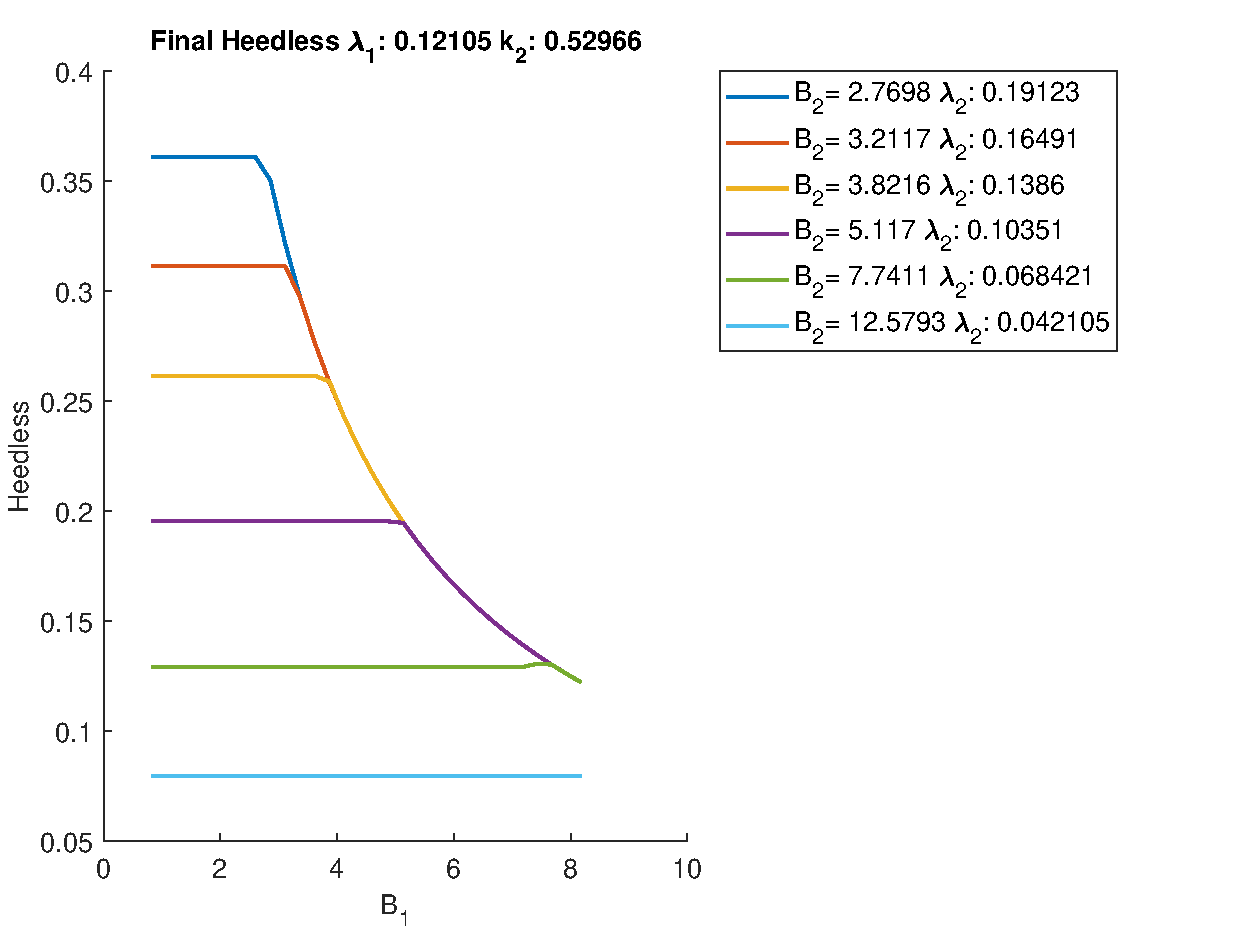
\includegraphics[width=.48\textwidth]{1_corpo/figure/behavioural_equilibrium/final_heedless_B1}}
	\caption[Final Behavioural variables varying $\mathcal{B}_1$]{The asymptotic value reached at the equilibrium by every variable in the behavioural model as a function of $\mathcal{B}_1$ for different $\mathcal{B}_2$ values.}
	\label{fig:subfig_sensitivity_behavioural_r1}
\end{figure}
The plots show how, for a fixed values of $\lambda_1$,$\lambda_2$ and $k_2$, the equilibrium value of the variables changes when varying the $k_1$ coefficient. To highlight the threshold effect due to the comparison of reproduction rates, the x-axis reports $\mathcal{B}_1$, which can be calculated knowing the value of  $\lambda_1$ and $k_1$. For the same reason, different $\mathcal{B}_2$ are considered. 

The threshold effect is clearly visible here as well. When examining the final values for the Compliant and Against variables, it is evident that once the $\mathcal{B}_1$ reproductive coefficient becomes dominant, the increase in the final size observed in the Compliant variable results from a decrease in the Against variable.

\subsubsection{Heat map of peak values}
We consider the peak values reached by the Compliant and Against variables. Figure \ref{fig:max_against} illustrates the maximum value reached by the Against variable. Instead, Figure \ref{fig:max_against2} shows the evolution of Against, in different simulations where $k_1, k_2, \lambda_1$ are kept constant, and different $\lambda_2$ are considered.
In both Figures, two situations are compared: in the first, $k_1 \sim k_2$, while in the other the difference between the two parameters is higher. Figure \ref{fig:max_against} shows three possible situations:

\begin{itemize}
	\item $\mathcal{B}_2 > \mathcal{B}_1$, and the maximum value corresponds to the value at the Equilibrium. It is the bottom right part of the picture.
	\item $\mathcal{B}_2 < \mathcal{B}_1$, but $\lambda_2 > \lambda_1$. These cases are located on the diagonal threshold of the heat map, and are the situations in which there is first a peak of $A$, but then $C$ is the dominant group at the equilibrium.
	\item $\mathcal{B}_2 < \mathcal{B}_1$ and also $\lambda_2 < \lambda_1$. Here there is no peak, and $A$ tends always to zero, or remain approximately zero, depending on the initial conditions. It is the top left part of pictures. 
\end{itemize}

In Figure \ref{fig:max_against}a, \(k_1 \sim k_2\), and the heatmap clearly shows the threshold effect when \(\mathcal{B}_1\) becomes larger than \(\mathcal{B}_2\). The transition of the peak value is not as abrupt as the one shown in Figure \ref{fig:subfig_sensitivity_behavioural}, as it reflects scenarios where there is a peak of \(A\) before reaching the asymptotic value.
These scenarios are similar to those presented in Case IV of the simulation discussed earlier in Section \ref{par:behav_4_case}.
 Figure \ref{fig:max_against2}a illustrates examples of scenarios that follows this change in the dynamics: depending on the considered value of \(\lambda_2\), the evolution of \(A\) varies. In certain scenarios, \(A\) becomes dominant, while in others, it shows a peak and then tends toward zero.


Figures \ref{fig:max_against}b, \ref{fig:max_against2}b represent the situation with $k_2 \gg k_1$. Here the Against is always dominant for every combination of $\lambda_1, \lambda_2$.
The red vertical line, called "section line" in Figure \ref{fig:max_against}, represents the part of the heat map, with the same parameters values used in the simulation in Figure \ref{fig:max_against2}.

\begin{figure}
	\centering
	\subfloat[][Maximum value of the Against variable with $k_1 \sim k_2 $]
	{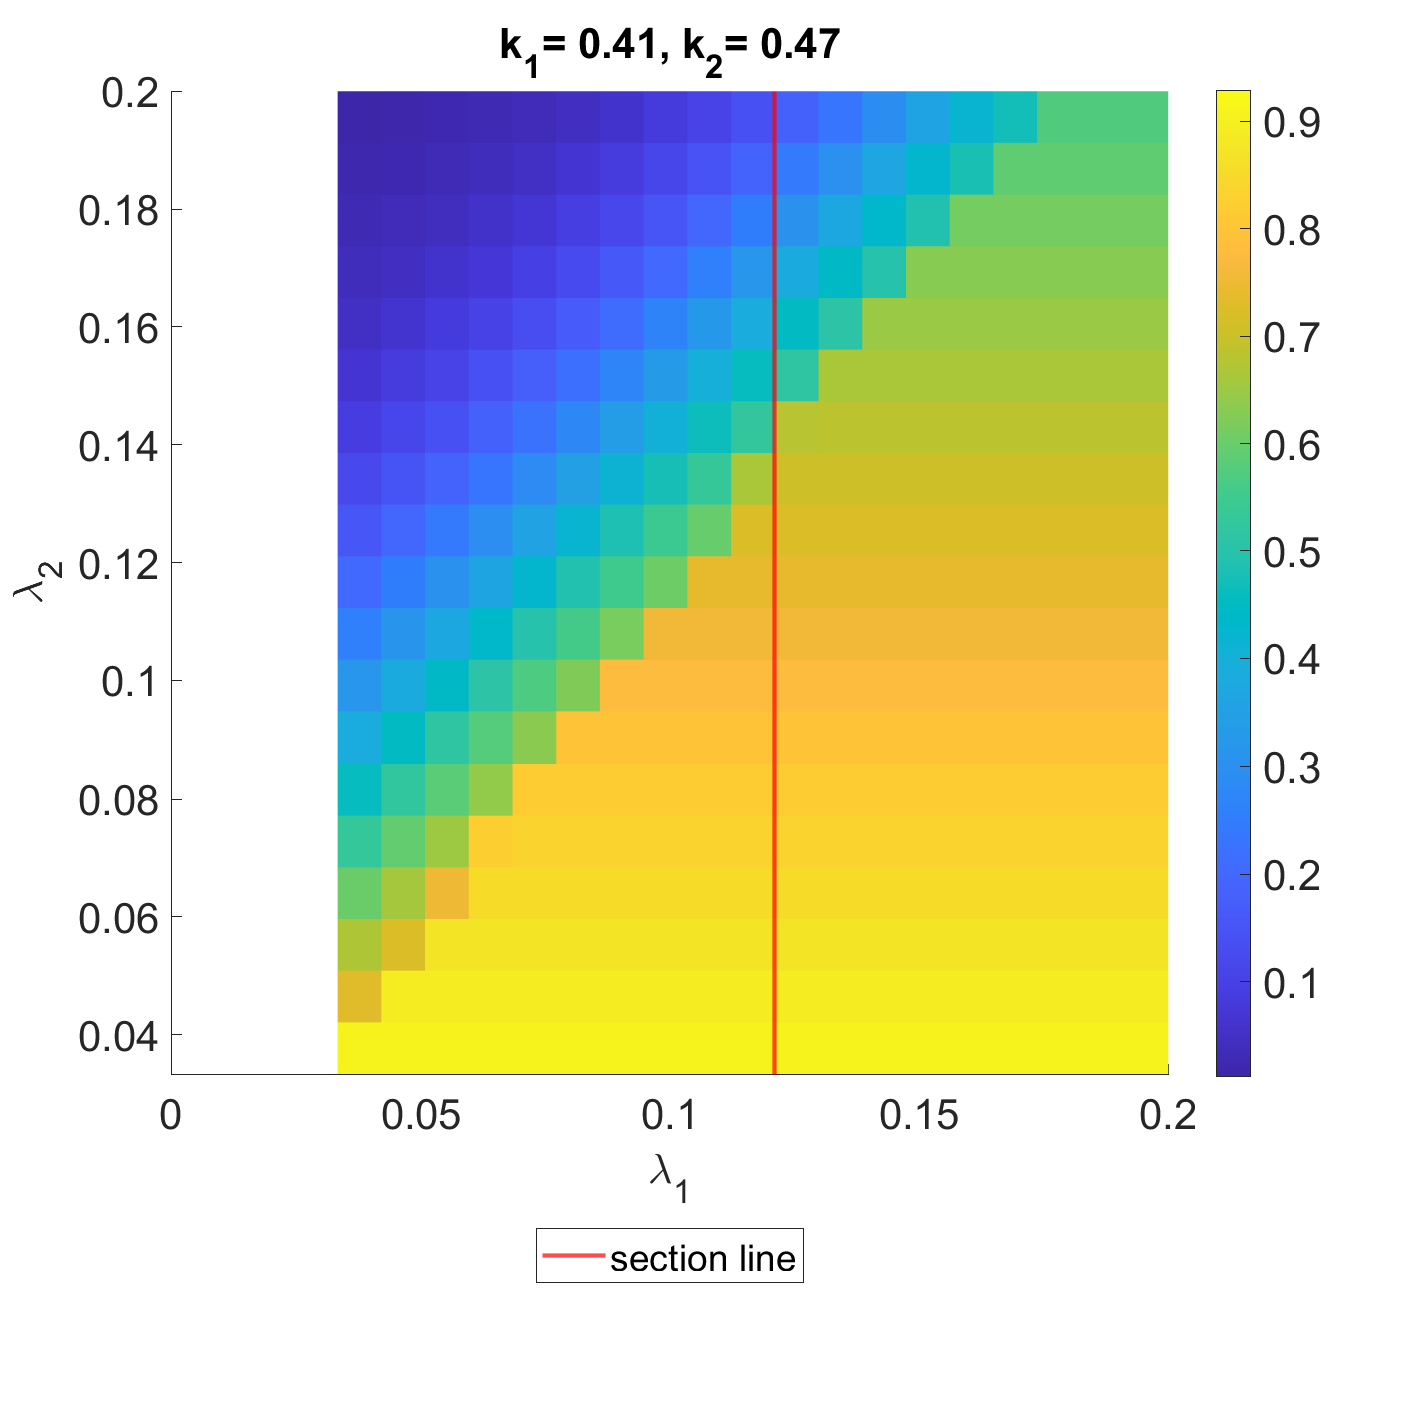
\includegraphics[width=.48\textwidth, valign= t]{1_corpo/figure/behavioural_equilibrium/max_againste_heatmap_1}} \quad
	\subfloat[][Maximum value of the Against variable with $k_1 < k_2 $]
	{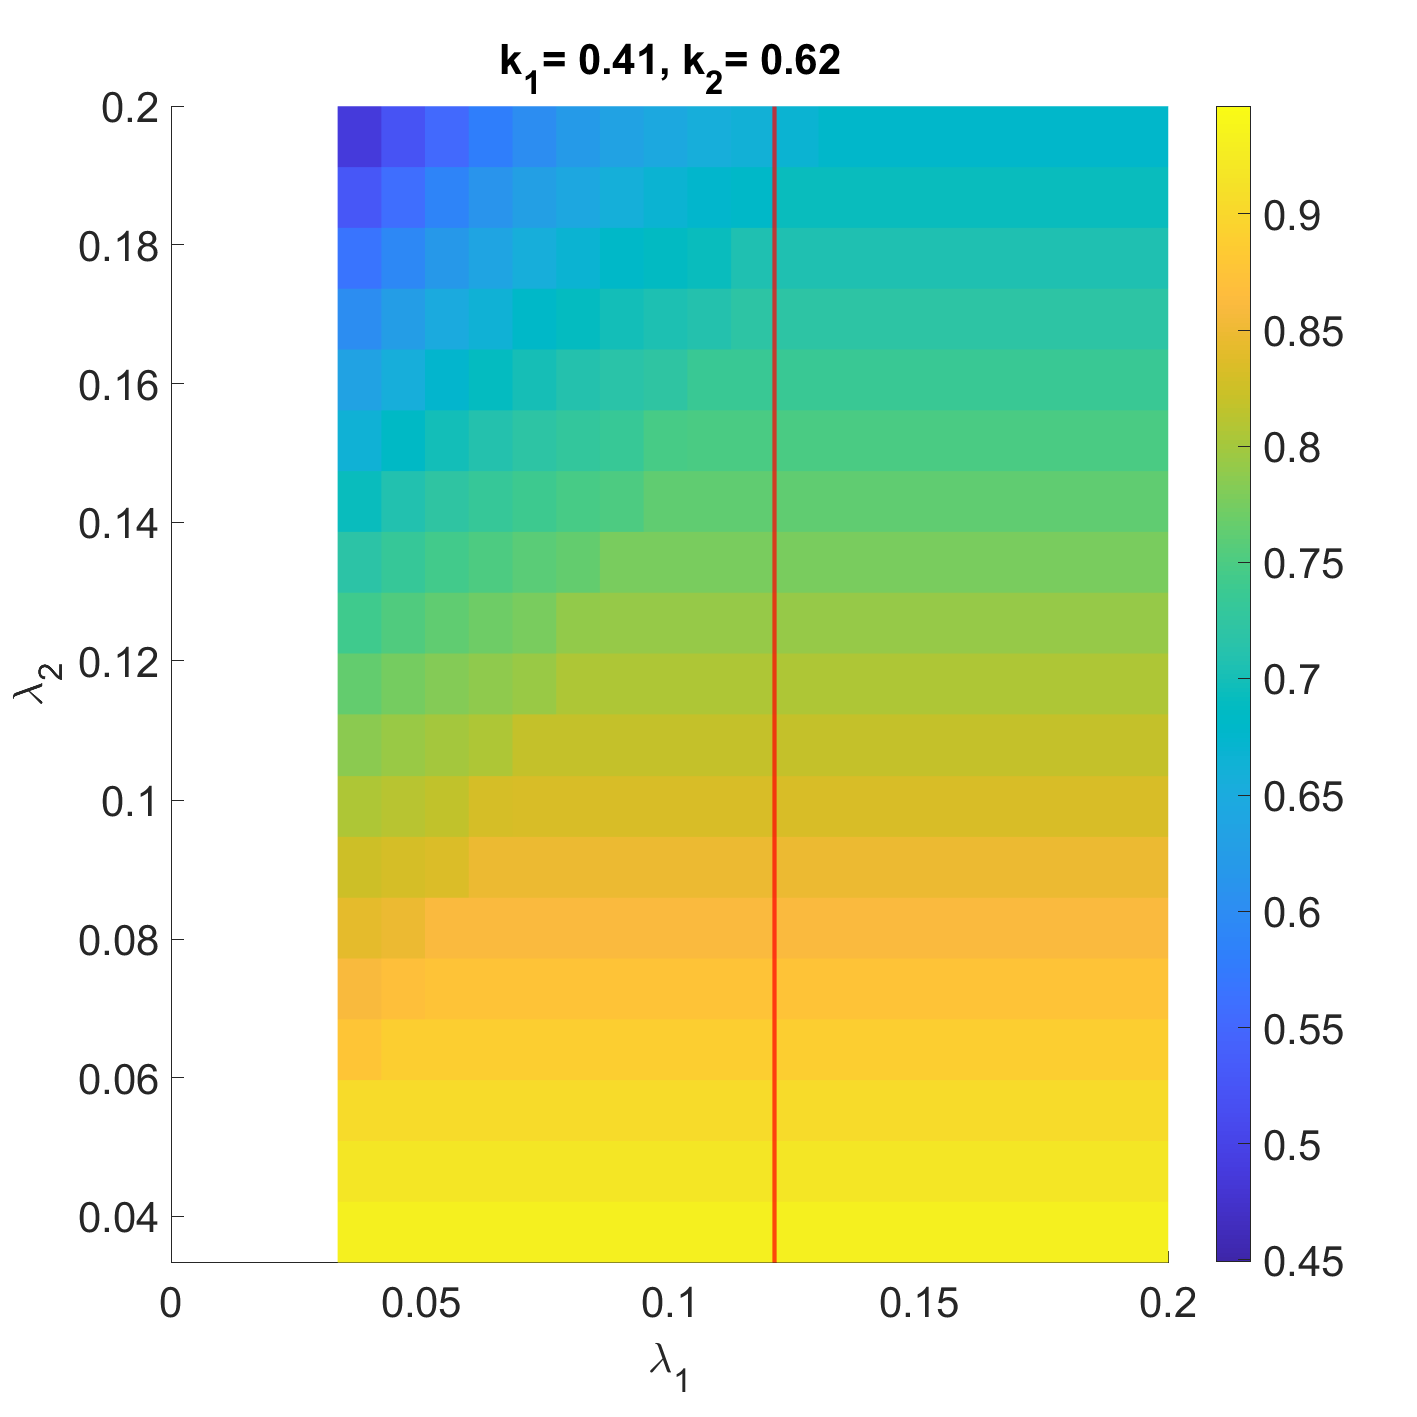
\includegraphics[width=.48\textwidth, valign= t]{1_corpo/figure/behavioural_equilibrium/max_againste_heatmap_2}} \\
	\caption[Maximum Against]{ The peak value of Against variable varying the $\lambda_1, \lambda_2$.}
	\label{fig:max_against}
\end{figure}

\begin{figure}
	\centering
	\subfloat[][Against simulation, with $k_1 \sim k_2$.]
	{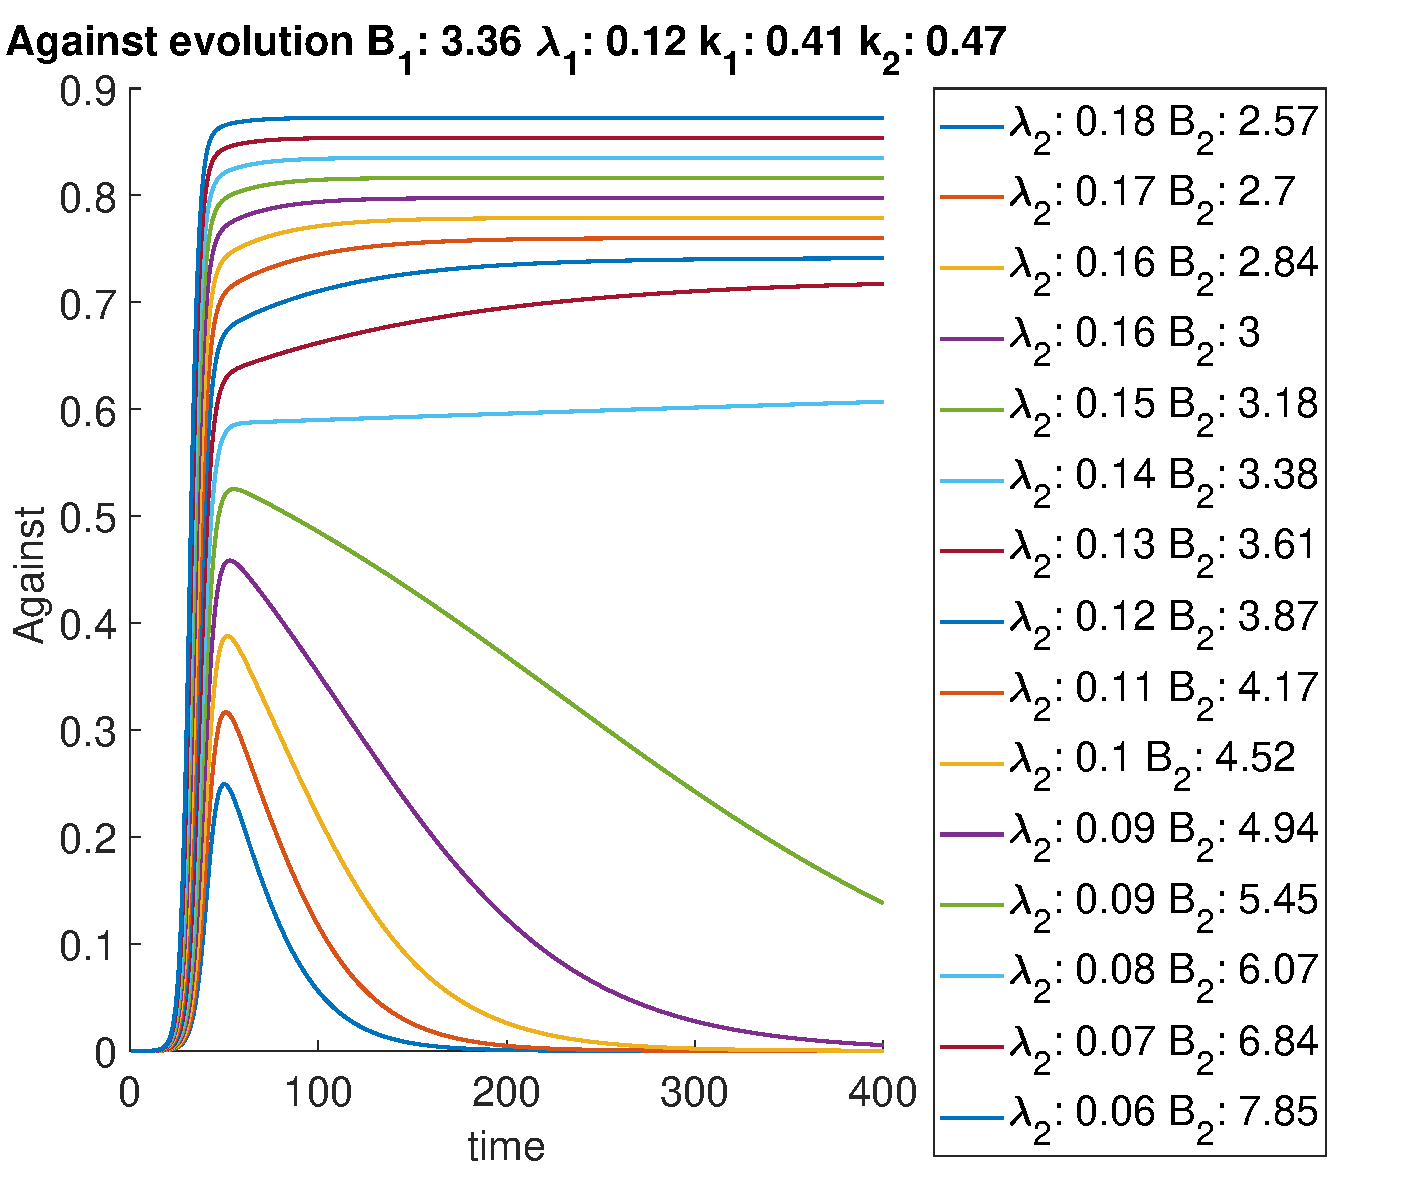
\includegraphics[width=.48\textwidth]{1_corpo/figure/behavioural_equilibrium/against_evolution_vari_1}} \quad
	\subfloat[][Against simulation, with $k_2 \gg k_1$.]
	{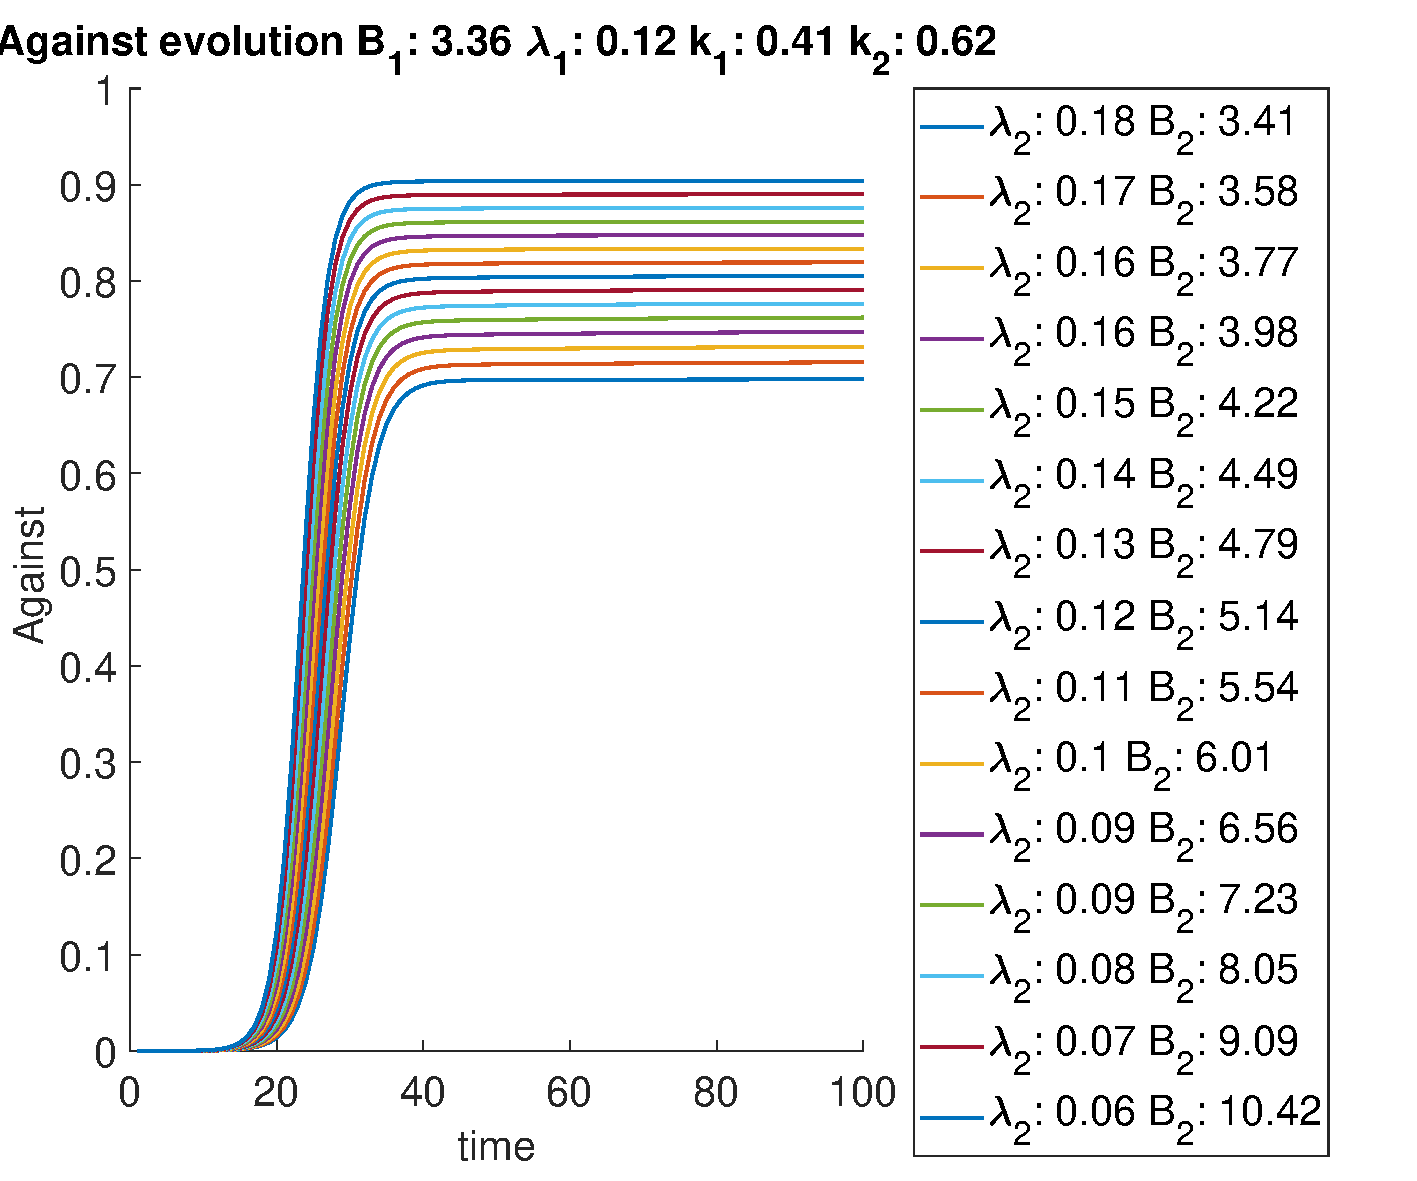
\includegraphics[width=.48\textwidth]{1_corpo/figure/behavioural_equilibrium/against_evolution_vari_2}} \\
		\caption[Max against first case]{The evolution of the Against variable, fixing $k_1, \lambda_1$, and $k_2$ and varying only  $\lambda_2$.}
	\label{fig:max_against2}
\end{figure}

\subsubsection{Conclusions}


In this chapter, we have introduced the SIRS model and conducted an in-depth study of the behavioral model. We have outlined the modeling choices underlying its design and analyzed the system's possible evolutions both analytically and through simulations. 

The key findings from the behavioral model analysis are as follows:  
\begin{itemize}
	\item For a behavior to spread within the population, its transmission rate, \( k_i \), must exceed the fatigue associated with maintaining it, \( \lambda_i \), where \( i = 1, 2 \). This condition translates into requiring the reproduction conversion number to be greater than one, \( \mathcal{B}_i > 1 \).  
	\item When two opposing behaviors coexist in the same system, if both have \( \mathcal{B}_i > 1 \), the behavior with the higher \( \mathcal{B}_i \) value becomes dominant asymptotically, while the other behavior diminishes to negligible levels.  
	\item If the two behaviors have the same \( \mathcal{B}_i \) value, the initial proportions of Compliant and Against individuals in the population determine the final distribution, as the influxes and outfluxes between the compartments tend to balance each other.  
	\item A behavior may have a lower reproduction conversion number, \( \mathcal{B}_i \), than the other, yet exhibit a higher \( k_i \) and \( \lambda_i \). For example, consider the case where \( k_1 = 0.1 \), \( \lambda_1 = 0.01 \), and \( k_2 = 0.3 \), \( \lambda_2 = 0.15 \). The corresponding conversion numbers are \( \mathcal{B}_1 = \frac{k_1}{\lambda_1} = 10 \) and \( \mathcal{B}_2 = 2 \). In this scenario, the system does not immediately converge to the behavior associated with \( \mathcal{B}_1 \). Instead, due to the higher transmission rate \( k_2 \), behavior 2 initially spreads at the expense of behavior 1. Over time, however, behavior 2's high fatigue cost (\( \lambda_2 \)) leads individuals to abandon it in favor of behavior 1, which is less attractive but also much less hard to sustain. This situation can be interpreted as a transitory popular trend, where a rapidly adopted behavior eventually gives way to a more stable alternative.  
\end{itemize}  

The insights gained here form the foundational toolkit required to accurately interpret the results arising from coupling the SIRS model with the behavioral model. In the next chapter (\ref{ch:epi_behav_model}), we present the design and the results of this coupling.
